%\documentclass[a4paper,12pt,twoside]{book}
\documentclass[listof=nochaptergap,12pt,times,authoryear]{report}
\usepackage{mathptmx}%This package supersedes times and mathptm
\usepackage[a4paper,right=2.54cm,left=2.54cm,top=2.54cm,bottom=2.54cm]{geometry}
\usepackage{array}
\usepackage{listings}
\usepackage{pdflscape}
\usepackage{longtable}
\usepackage{enumitem}
\usepackage{newclude}
\usepackage{float}
\usepackage{comment}
\usepackage[export]{adjustbox}
\usepackage{algorithm}
\usepackage{algpseudocode}

\floatname{algorithm}{Algoritmo}

\newcolumntype{C}[1]{>{\centering\arraybackslash}p{#1}}
\newcolumntype{N}{@{}m{0pt}@{}}
\newcommand\fillin[1][3cm]{\makebox[#1]{\dotfill}}

%%Paquete para ocultar indices de tabla de contenidos
%% Numeración continua en figuras y tablas
\setcounter{equation}{0}
\usepackage{chngcntr}
\counterwithout{figure}{chapter}
\counterwithout{table}{chapter}
\counterwithout{equation}{chapter}
\renewcommand{\thefigure}{\arabic{figure}}
\renewcommand{\thetable}{\arabic{table}}
\renewcommand{\theequation}{\arabic{equation}}

% Parche para eliminar espacios por capítulos en lista de figuras y tablas
\usepackage{etoolbox}% http://ctan.org/pkg/etoolbox
\makeatletter
% \patchcmd{<cmd>}{<search>}{<replace>}{<succes>}{<failure>}
\patchcmd{\@chapter}{\addtocontents{lof}{\protect\addvspace{10\p@}}}{}{}{}% LoF
\patchcmd{\@chapter}{\addtocontents{lot}{\protect\addvspace{10\p@}}}{}{}{}% LoT
\makeatother


%%%%paquete para usar citas de diferentes formatos
%%%%%%%%%%%%%%%%%%%%%%%%%%%%%%%%%
%%add al indice
%\usepackage[nottoc,numbib]{tocbibind}
%\usepackage[authoryear,round]{natbib}
\usepackage[utf8]{inputenc}
\usepackage{csquotes}
\usepackage[spanish,es-lcroman]{babel}
\decimalpoint
%% Citas y bibliografía formato APA
\usepackage[backend=biber,style=apa,natbib=true]{biblatex}
%\DeclareLanguageMapping{australian}{australian-apa}
\DeclareLanguageMapping{spanish}{spanish-apa}
\addbibresource{biblio/references.bib}

%% Formato DOI
\DeclareFieldFormat{doi}{%
	doi\addcolon\space
	\ifhyperref
	{\lowercase{\href{https://doi.org/#1}{\nolinkurl{#1}}}}
	{\lowercase{\nolinkurl{#1}}}}

%% Formato de URL en referencias
\DeclareFieldFormat{url}{{Recuperado de}\space\url{#1}}

%% Convertir comando cita por textcite para que tenga formato APA
\let\cite\textcite

%% Para que texto de figuras y tablas tenga formato APA
\usepackage{multirow,booktabs,setspace,caption}
\DeclareCaptionLabelSeparator*{spaced}{\\[2ex]}
\captionsetup[table]{labelfont=normalfont,textfont=it,format=plain,justification=justified,singlelinecheck=false,labelsep=newline,skip=2pt}
\captionsetup[figure]{labelsep=period,labelfont={it,bf},justification=justified,singlelinecheck=false,font=doublespacing}
\captionsetup[subfigure]{justification=centering}

%%%Editar formato y tamaño de capítulos y secciones
\usepackage{titlesec}
\titleformat{\chapter}
{\centering\normalfont\large\bfseries}{Capítulo \thechapter:}{1em}{}
\titlespacing*{\chapter}{0pt}{-4ex}{1ex}

\titleformat{\section}
{\normalfont\large\bfseries}{\thesection}{1em}{}
\titlespacing*{\section}{0pt}{0pt}{0pt}

\titleformat{\subsection}
{\normalfont\large\bfseries}{\thesubsection}{1em}{}
\titlespacing*{\subsection}{0pt}{0pt}{0pt}

%\usepackage{biblatex}
%paquete para hiperlinks entre citas e imagenes
%%%%%%%%%%%%%%%%%%%%%%%%%%%%%%%%%
\usepackage[colorlinks=true,
citecolor=black,
urlcolor=black,
bookmarks=true,
linkcolor=black,
pdftitle={Tesis-nombre-alumno},
pdfauthor={autor nombres}]{hyperref}

\usepackage{amssymb}
\usepackage{graphicx} % for improved inclusion of graphics
%\usepackage{wrapfig} % to include figure with text wrapping around it
\usepackage[margin=10pt,font=small,labelfont=bf]{caption} % for improved layout of figure captions with extra margin, smaller font than text
\usepackage{subcaption}
\usepackage{eucal}
\usepackage[usenames, dvipsnames]{color}
\usepackage[perpage]{footmisc}
%\usepackage[round, sort]{natbib}
\usepackage{ifthen}
\usepackage{multicol} % for pages with multiple text columns, e.g. References
\setlength{\columnsep}{20pt} % space between columns; default 10pt quite narrow
%% Para no mostrar índices de figuras ni tablas en el índice general
\usepackage[nottoc,notlot,notlof]{tocbibind}
%\usepackage{appendix}
\usepackage[titletoc,title]{appendix} 

%%%----Modificar encabezado y pie de pagina
%%%%%%%%%%%%%%%%%%%%%%%%%%%%%%%%%%%%%%%%%%%%%%%%%%%%%%%%%%%%%%%%%%%%%
\usepackage{fancyhdr} % for better header layout
\newcommand{\changefont}{%
	\fontsize{9pt}{1.5pt}\selectfont
}

\pagestyle{fancy}
%%Para borrar fancy por default (incluye numeracion)
\fancyhf{} % sets both header and footer to nothing
%%Para borrar linea de encabezado
\renewcommand{\headrulewidth}{0pt}
%%Encabezados solo con numero de pagina
\fancypagestyle{normal}{%
	\fancyhead{} % clear all header fields
	\fancyhead[R]{\thepage}}
%%Encabezados con titulo de tesis y numero de pagina
\fancypagestyle{special}{%
	\fancyhead[L]{\changefont Desarrollo de una aplicación móvil para el prediagnóstico de bruxismo en niños utilizando técnicas de aprendizaje profundo
	}
	\fancyhead[R]{\thepage}}


%\fancyhf{} %% delete default configuration of page
%%\setlength\headheight{15pt}

%%%%%%%%%%%%%%%%%%%%%%%%%%%%%5
%%%% Configuracion de los parrafos
%\usepackage{setspace}
%\onehalfspacing
%\linespread{1.25} 
\setlength{\parindent}{0.5in} %%sangria
\setlength{\parskip}{3mm}  %%espacio entre parrafos
\linespread{1.3} %This equals 1.5 linespacing in Word
%%%% nuevo parrafo
%%%%%%%%%%%%%%%%%%%%%%%%%%%%%5
%%%% Centrar valores de una tabla
\usepackage{array}
%%CENTRADO HORIZONTAL
\newcolumntype{P}[1]{>{\centering\arraybackslash}p{#1}}
%%CENTRADO VERTICAL
\newcolumntype{M}[1]{>{\centering\arraybackslash}m{#1}}

%%%%%%%%%%%%%%%%%%%%%%%%%%%%%5
%%%%Paquete para alinear texto
\usepackage{ragged2e}
\usepackage{multirow}
\usepackage{makecell}
\usepackage{rotating}
\usepackage{siunitx} % To align the numbers later on
\usepackage[table,xcdraw]{xcolor}
\usepackage{color, colortbl}
\definecolor{Gray}{gray}{0.9}
\definecolor{orange}{rgb}{1,0.647,0}
\definecolor{turq3}{rgb}{0.54, 0.81, 0.94}
\definecolor{turq}{rgb}{0.63, 0.79, 0.95}
\definecolor{bluejean}{rgb}{0.03, 0.27, 0.49}

%%%%%%%%%%%%%%%%%%%%%%%%%
\usepackage{xparse}
\usepackage{expl3}
%%%%funcion de reemplazar regex
\ExplSyntaxOn
\NewDocumentCommand{\replace}{mmm}
{
	\marian_replace:nnn {#1} {#2} {#3}
}

\tl_new:N \l_marian_input_text_tl
\tl_new:N \l_marian_search_tl
\tl_new:N \l_marian_replace_tl

\cs_new_protected:Npn \marian_replace:nnn #1 #2 #3
{
	\tl_set:Nn \l_marian_input_text_tl { #1 }
	\tl_set:Nn \l_marian_search_tl { #2 }
	\tl_set:Nn \l_marian_replace_tl { #3 }
	\regex_replace_all:nnN { \b\u{l_marian_search_tl}\b } { \u{l_marian_replace_tl} } \l_marian_input_text_tl
	\tl_use:N \l_marian_input_text_tl
}
\ExplSyntaxOff

%%%%%%%%%%%%%%%%%%%%%%%%%%%%%%%%%%%%%%
\usepackage{amsmath}
%\setcounter{equation}{0}
%\numberwithin{equation}{chapter} %%enumerar ecuaciones
%\renewcommand{\theequation}{Ecuación \arabic{equation}}   
\usepackage{mathtools, nccmath, cool}
%%%Configuraciones de biblatex

%%%hel
%%%%\citeauthor
\makeatletter

%%%%%%%%%%%%
\DeclareCiteCommand{\citeauthor}
{\boolfalse{citetracker}%
	\boolfalse{pagetracker}%
	\usebibmacro{prenote}}
{\ifciteindex
	{\indexnames{labelname}}
	{}%
	\printtext[bibhyperref]{\printnames{labelname}}}
{\multicitedelim}
{\usebibmacro{postnote}}


\DeclareCiteCommand{\citetitle}
{\boolfalse{citetracker}%
	\boolfalse{pagetracker}%
	\usebibmacro{prenote}}
{\ifciteindex
	{\indexfield{indextitle}}
	{}%
	\printtext[bibhyperref]{\printfield[citetitle]{labeltitle}}}
{\multicitedelim}
{\usebibmacro{postnote}}

\DeclareCiteCommand{\cite}
{\usebibmacro{prenote}}
{\usebibmacro{citeindex}%
	\printtext[bibhyperref]{\usebibmacro{cite}}}
{\multicitedelim}
{\usebibmacro{postnote}}

\DeclareCiteCommand*{\cite}
{\usebibmacro{prenote}}
{\usebibmacro{citeindex}%
	\printtext[bibhyperref]{\usebibmacro{citeyear}}}
{\multicitedelim}
{\usebibmacro{postnote}}

\DeclareCiteCommand{\parencite}[\mkbibparens]
{\usebibmacro{prenote}}
{\usebibmacro{citeindex}%
	\printtext[bibhyperref]{\usebibmacro{cite}}}
{\multicitedelim}
{\usebibmacro{postnote}}

\DeclareCiteCommand*{\parencite}[\mkbibparens]
{\usebibmacro{prenote}}
{\usebibmacro{citeindex}%
	\printtext[bibhyperref]{\usebibmacro{citeyear}}}
{\multicitedelim}
{\usebibmacro{postnote}}

\DeclareCiteCommand{\footcite}[\mkbibfootnote]
{\usebibmacro{prenote}}
{\usebibmacro{citeindex}%
	\printtext[bibhyperref]{ \usebibmacro{cite}}}
{\multicitedelim}
{\usebibmacro{postnote}}

\DeclareCiteCommand{\footcitetext}[\mkbibfootnotetext]
{\usebibmacro{prenote}}
{\usebibmacro{citeindex}%
	\printtext[bibhyperref]{\usebibmacro{cite}}}
{\multicitedelim}
{\usebibmacro{postnote}}

\DeclareCiteCommand{\textcite}
{\boolfalse{cbx:parens}}
{\usebibmacro{citeindex}%
	\printtext[bibhyperref]{\usebibmacro{textcite}}}
{\ifbool{cbx:parens}
	{\bibcloseparen\global\boolfalse{cbx:parens}}
	{}%
	\multicitedelim}
{\usebibmacro{textcite:postnote}}
\makeatother
\makeatletter
\let\abx@macro@citeOrig\abx@macro@cite
\renewbibmacro{cite}{%
	\bibhyperref{%
		\let\bibhyperref\relax\relax%
		\abx@macro@citeOrig%
	}%
}
\let\abx@macro@textciteOrig\abx@macro@textcite
\renewbibmacro{textcite}{%
	\bibhyperref{%
		\let\bibhyperref\relax\relax%
		\abx@macro@textciteOrig%
	}%
}%

\makeatother

%%%%%%%%%%%%%%%%%%%%%%%%%%%%%%%%%%%%%%%%%%%
% Agregando librerias para que aparezca texto debajo de las ecuaciones.
\usepackage[titles]{tocloft}

%% Para agregar palabra "CAPÍTULO" en 
\newlength\mynewlength
\let\oldcftchappresnum\cftchappresnum
\renewcommand*\cftchappresnum{Capítulo \oldcftchappresnum}
\renewcommand\cftchapaftersnum{:}
\settowidth\mynewlength{\cftchappresnum\cftchapaftersnum\quad}
\addtolength\cftchapnumwidth{\mynewlength}

\usepackage{xpatch}
\usepackage{caption}
\DeclareCaptionType{equcaption}[Ecuación][Índice de Ecuaciones]

\newenvironment{conditions}
{\par\vspace{\abovedisplayskip}\noindent\begin{tabular}{>{$}l<{$} @{${}={}$} l}}
	{\end{tabular}\par\vspace{\belowdisplayskip}}

% Para agregar linea de puntos en la tabla de contenidos
\renewcommand{\cftpartleader}{\cftdotfill{\cftdotsep}} % for parts
\renewcommand{\cftchapleader}{\cftdotfill{\cftdotsep}} % for chapters

% Para eliminar linea de puntos de la tabla de contenidos
%\renewcommand{\cftdot}{}

% Para alinear párrafo en indice de figuras y tablas
\cftsetindents{figure}{0em}{2.5em}
\renewcommand\cftfigpresnum{\figurename~}
\renewcommand{\cftfigaftersnum}{.} % Goes after figure number
\newlength\mylength
\settowidth\mylength{\cftfigpresnum}
\addtolength\cftfignumwidth{\mylength}
\cftsetindents{table}{0em}{2.5em}
\renewcommand\cfttabpresnum{Tabla }
\renewcommand{\cfttabaftersnum}{.} % Goes after figure number
\settowidth\mylength{\cfttabpresnum}
\addtolength\cfttabnumwidth{\mylength}

\DefineBibliographyExtras{spanish}{%
	\savecommand\sptext
	\renewcommand*{\sptext}{\textsuperscript}}

\UndefineBibliographyExtras{spanish}{%
	\restorecommand\sptext}

%%Formato APA (No funciona en biblatex)
\usepackage{apalike}
%\bibliographystyle{apalike}

\begin{document}
% Se añade esto para agregar la lista de ecuaciones en el indice del documento	

\newcommand{\listequationsname}{Índice de Ecuaciones}
\newlistof{myequations}{equ}{\listequationsname}
\newcommand{\myequations}[1]{%
	\addcontentsline{equ}{myequations}{Ecuación \protect\numberline{\theequation}#1}\par}
%\addcontentsline{toc}{section}{Índice de Ecuaciones}

%%Numeros de pagina en romano (minuscula)
%\pagenumbering{roman}
\renewcommand{\thepage}{\roman{page}}

% Beginning of hack...
%\let\oldthispagestyle=\thispagestyle % If we want to see a page number.
%\def\thispagestyle#1{} % If we want to see a page number.
%\let\oldsetcounter=\setcounter
%\def\setcounter#1#2{}
% End of hack...

\begin{titlepage}

	\begin{center}
		%%%cargar imagen
	    
\includegraphics[width=0.20\textwidth]{images_repo/esanlogomin}
		\vspace*{2cm} \\
		UNIVERSIDAD ESAN \vspace*{1ex} \\
		FACULTAD DE INGENIERÍA \vspace*{1ex} \\
		INGENIERÍA DE TECNOLOGÍAS DE INFORMACIÓN Y SISTEMAS
		\vspace*{8ex} \\
		%\textbf
		{Desarrollo de una aplicación móvil para el prediagnóstico de bruxismo en niños utilizando técnicas de aprendizaje profundo
		}
		\vspace*{8ex}\\	
		Tesis de investigación para el curso Trabajo de Tesis I 
		\vspace*{8ex} \\	
		Anderson Richard Calloquispe Ccoya\\
		Asesor: Marks Calderón		
		\vfill
		Lima, \today 
		
	\end{center}
\end{titlepage}
%%Permite mostrar encabezado y numeracion en primera pagina de capitulos - indices
\fancypagestyle{plain}{}
%%cambiar nombres de objetos para el indice y otros
\renewcommand{\listfigurename}{Índice de Figuras}
\renewcommand{\tablename}{Tabla}
\renewcommand{\listtablename}{Índice de Tablas}
\renewcommand{\listalgorithmname}{Índice de Algoritmos}

%%Permite empezar conteo de paginas de forma personalizada
\addtocounter{page}{1}
\pagestyle{normal}
%\thispagestyle{plain}
%\vspace{0.5cm}
\leftline{Esta tesis denominada:}
\begin{center}
	%\vspace*{10cm}
	{DESARROLLO DE UNA APLICACIÓN MÓVIL PARA EL PREDIAGNÓSTICO DE BRUXISMO EN NIÑOS UTILIZANDO TÉCNICAS DE APRENDIZAJE PROFUNDO}
\end{center}

\leftline{ha sido aprobada.}
\vspace{3cm}

%\dotfill
\rightline{\fillin[9cm]}
\rightline{Jurado 1}
\vspace{3cm}

%\dotfill
\rightline{\fillin[9cm]}
\rightline{Jurado 2}
\vspace{3cm}

%\dotfill
\rightline{\fillin[9cm]}
\rightline{Jurado 3}
\vspace{3cm}

\centerline{Universidad ESAN}
\centerline{2024}
%\thispagestyle{plain}
\begin{center}
	\vspace*{10cm}
	{Desarrollo de una aplicación móvil
	para el prediagnóstico de bruxismo
	en niños utilizando técnicas de
	aprendizaje profundo}
	
\end{center}

%\thispagestyle{plain}
\begin{center}
	%\vspace*{1.5cm}
	{\large \bfseries  Dedicatoria}
\end{center}
\vspace{0.5cm}

A mis padres.

Gracias por su gran apoyo a traves de los años.
\newline



% outline
\tableofcontents            % print the table of contents

%: ----------------------- contents ------------------------

\setcounter{secnumdepth}{3} % organisational level that receives a numbers
\setcounter{tocdepth}{3}    % print table of contents for level 3

% levels are: 0 - chapter, 1 - section, 2 - subsection, 3 - subsection


%: ----------------------- list of figures/tables ------------------------
\clearpage
\listoffigures
\clearpage
\listoftables  % print list of tables
\clearpage
\phantomsection
%\listofequcaptions % print list of equations
\listofmyequations
\clearpage
\listofalgorithms
\clearpage
%% Numeros de pagina en arabic (si se desea continuar la numeración)
%\renewcommand{\thepage}{\arabic{page}}
%% Para reiniciar la numeración
\pagenumbering{arabic}
%%Encabezado con titulo de tesis y numeracion
\pagestyle{special}
%La línea de abajo es para quitar encabezado
%\thispagestyle{plain}

\chapter*{Resumen}
\markboth{Resumen}{Resumen}
\addcontentsline{toc}{chapter}{Resumen}

%RESUMEN
Con el incremento de casos de bruxismo infantil en los últimos años, especialistas en odontología e investigadores han identificado la necesidad de desarrollar métodos confiables y herramientas eficaces que permitan a los profesionales de la salud detectar y diagnosticar esta condición en etapas tempranas. Esto es especialmente relevante en contextos de clínicas u hospitales con recursos limitados y con acceso reducido a personal especializado. Un diagnóstico tardío o impreciso puede derivar en complicaciones mayores, como desgaste dental severo, problemas musculares y articulares, e incluso trastornos en el desarrollo facial.

Por ello, y considerando los avances actuales en el campo de la Inteligencia Artificial junto con el creciente acceso a herramientas computacionales de alto rendimiento, esta investigación propone el desarrollo de una aplicación móvil basada en técnicas de aprendizaje profundo para el prediagnóstico de bruxismo en niños. La herramienta analizará imágenes de la lengua con marcas características asociadas a esta condición, mejorando la precisión y rapidez del diagnóstico al mismo tiempo que facilita su implementación en entornos con recursos limitados.


\textbf{Palabras claves: } Aprendizaje profundo, Redes Neuronales Convolucionales, Visión por Computadora, imágenes, bruxismo, niños.

\clearpage
%\vspace{0.5cm}
\chapter*{Abstract}
\markboth{Abstract}{Abstract}

%LOMISMO PERO EN INGLES
With the increasing prevalence of bruxism in children in recent years, dental specialists and researchers have recognized the need to develop reliable methods and effective tools to enable healthcare professionals to detect and diagnose this condition at early stages. This is particularly important in clinics or hospitals with limited resources and reduced access to specialized personnel. Late or inaccurate diagnoses can lead to severe complications, such as advanced dental wear, muscular and joint problems, and even facial development disorders.

In light of this, and considering the current advancements in Artificial Intelligence along with the growing accessibility to high-performance computational tools, this research proposes the development of a mobile application based on deep learning techniques for the prediagnosis of bruxism in children. The tool will analyze tongue images with specific marks associated with this condition, improving the accuracy and speed of diagnosis while facilitating its implementation in resource-limited environments.


\textbf{Keywords: }Deep Learning, Convolutional Neural Networks, Computer Vision, tongue images, bruxism, children
%La línea de abajo es para quitar encabezado
%\thispagestyle{plain}

\chapter*{Introducción}
\markboth{Introducción}{Introducción}
\addcontentsline{toc}{chapter}{Introducción}
% texto 
El principal objetivo de la presente investigación es desarrollar y proponer un modelo basado en inteligencia artificial para el prediagnóstico rápido y preciso del bruxismo en niños. Esto se logrará mediante la clasificación de imágenes de lengua con marcas características asociadas a esta condición. Para ello, se utilizarán algoritmos avanzados del campo del aprendizaje profundo. En particular, se implementarán Redes Neuronales Convolucionales (CNNs) y Vision Transformers, herramientas reconocidas por su capacidad de identificar patrones en imágenes y que serán clave para este proyecto.

Las imágenes de lengua que se emplearán para el entrenamiento y validación de los modelos serán extraídas de bases de datos en línea debidamente verificadas, asegurando su validez científica. El proceso de desarrollo incluirá una etapa inicial de preprocesamiento y selección de imágenes, con el objetivo de crear un conjunto de datos óptimo para el modelado. Posteriormente, se implementarán distintos algoritmos y técnicas dentro del ámbito del Deep Learning, evaluándose su desempeño mediante métricas específicas. Esto permitirá seleccionar el modelo más eficiente y eficaz, como se detalla en la metodología de la implementación.

La herramienta de inteligencia artificial que se desarrollará no busca reemplazar el diagnóstico clínico de un profesional especializado, sino convertirse en un recurso de apoyo que facilite la detección temprana de bruxismo. Esto es crucial, ya que un diagnóstico adecuado en etapas iniciales puede prevenir complicaciones graves como desgaste dental severo, dolores musculares, e incluso problemas articulares o de desarrollo facial.

El problema central que se aborda en esta investigación radica en la falta de herramientas tecnológicas específicas para el prediagnóstico de bruxismo en niños, especialmente en contextos con acceso limitado a especialistas. Además, el proceso de detección suele depender exclusivamente de la experiencia del profesional, lo que puede aumentar el margen de error o prolongar el diagnóstico. Este proyecto busca cerrar esta brecha mediante la aplicación de técnicas avanzadas de inteligencia artificial, aprovechando los recientes avances tecnológicos para ofrecer una solución eficiente y accesible.

La creciente preocupación por los problemas de bruxismo en niños, tanto en el Perú como a nivel mundial, impulsa esta investigación. Se espera que los resultados permitan mejorar los tiempos y la precisión en el diagnóstico, facilitando tratamientos oportunos y reduciendo complicaciones futuras en la salud bucodental infantil.
%\newcommand\chap[1]{%
%	\chapter*{#1}%
%	\addcontentsline{toc}{chapter}{#1}}


%%Num. de capitulos en romano y el resto en arabic
\renewcommand{\thechapter}{\Roman{chapter}}
\renewcommand{\thesection}{\arabic{chapter}.\arabic{section}}
\renewcommand{\thesubsection}{\arabic{chapter}.\arabic{section}.\arabic{subsection}}

% Este es el comando que funciona para las ecuaciones
\renewcommand{\theequcaption}{\arabic{equcaption}}

%%Para insertar los capítulos y agregando nueva página al terminar
%\chapter{Planteamiento del Problema}
\section{Descripción de la Realidad Problemática}

El bruxismo, definido como una actividad repetitiva de los músculos mandibulares que incluye el apretamiento o rechinamiento involuntario de los dientes, es una condición muy frecuente en la población infantil. De acuerdo con la Academia Americana de Medicina del Sueño, este hábito no controlado ocurre principalmente durante las horas de descanso nocturno y puede generar importantes repercusiones tanto en la salud bucal como en el bienestar general del niño \parencite{AmericanAcademy2014}.

La prevalencia de esta condición en niños es un tema ampliamente investigado, pero con resultados variables dependiendo de los contextos geográficos y los enfoques metodológicos utilizados en los estudios. Según una revisión sistemática, la prevalencia de bruxismo en niños menores de 12 años puede oscilar entre el 3.5\% y el 40.6\%, sin observarse diferencias significativas en cuanto a género \parencite{Manfredini2013}. En países de América Latina, como Brasil, los estudios indican cifras que varían entre un 32\% y un 43\%, mientras que en Chile se ha reportado una prevalencia cercana al 32\%, con un aumento hasta el 38\% en niños de 6 años \parencite{Shinkai1998, Sandoval2016}.

El bruxismo infantil puede clasificarse en dos categorías principales: bruxismo del sueño y bruxismo de vigilia. Aunque ambos tipos presentan características comunes, el bruxismo del sueño es más prevalente en niños, aunque frecuentemente pasa desapercibido en sus etapas iniciales. Esto dificulta su detección y tratamiento oportunos, incrementando el riesgo de complicaciones a largo plazo \parencite{Camoin2017}.

Diversos estudios destacan la naturaleza multifactorial del bruxismo infantil, identificando factores locales, psicológicos, hereditarios y fisiopatológicos como principales contribuyentes. Por ejemplo, las maloclusiones dentales, el estrés emocional y la ansiedad son factores recurrentes, mientras que una predisposición genética también juega un rol significativo. En particular, investigaciones han evidenciado que los niños cuyos padres tienen antecedentes de bruxismo presentan una mayor probabilidad de desarrollar esta condición \parencite{Abe1966, Lobbezoo1997}.

Una de las mayores dificultades en el diagnóstico del bruxismo en niños radica en distinguir entre el desgaste natural de los dientes asociado al desarrollo y el desgaste patológico provocado por esta condición. Los profesionales de la salud generalmente recurren a cuestionarios dirigidos a los padres para recopilar información, complementándolos con un examen clínico detallado del niño. Sin embargo, en casos más graves, la polisomnografía (PSG) se considera el estándar de oro para registrar los episodios de bruxismo durante el sueño \parencite{Luiz2008, Sandoval2016}. A pesar de su eficacia, la PSG presenta limitaciones significativas, como altos costos, infraestructura compleja y la incomodidad que genera en pacientes pediátricos \parencite{Chisini2020}.

Adicionalmente, estudios recientes han asociado el bruxismo con problemas respiratorios, como la apnea obstructiva del sueño (AOS), en la que los movimientos mandibulares pueden ser intentos del cuerpo para mejorar el flujo de aire durante el sueño \parencite{Bulanda2021, Goettems2017}. Estas conexiones subrayan la necesidad de métodos diagnósticos más accesibles y no invasivos. En este contexto, herramientas tecnológicas basadas en aprendizaje profundo, que analicen patrones como los movimientos mandibulares y las características observables en la lengua, podrían revolucionar la forma en que se diagnostica esta condición \parencite{Chisini2020}.

En Perú, los estudios reflejan cifras preocupantes. En La Brea, Piura, el 65.22\% de los niños entre 4 y 6 años presentan signos de bruxismo, con una mayor incidencia en niños de 5 años \parencite{Baldeon2014}. Asimismo, en Buenos Aires, Piura, se encontró una prevalencia de hasta el 69.8\% en niños preescolares \parencite{Delgado2002}. Estas cifras superan ampliamente las reportadas en países como Estados Unidos, donde la prevalencia alcanza el 38\% \parencite{Cheifetz2005}, o en Brasil, con un 43\% \parencite{Valera2003}.

Aunque factores como las parasitosis intestinales han sido objeto de estudio en relación con el bruxismo en Perú, no se ha hallado una correlación significativa \parencite{Baldeon2014}. Sin embargo, la alta prevalencia de esta condición justifica el desarrollo de soluciones tecnológicas innovadoras, como aplicaciones móviles basadas en aprendizaje profundo, para facilitar un diagnóstico temprano y más preciso.

En conclusión, el bruxismo infantil constituye una condición prevalente con múltiples factores etiológicos. Su diagnóstico oportuno es crucial para prevenir consecuencias graves, como desgaste dental severo, problemas musculares y articulares, así como alteraciones en el desarrollo facial. La implementación de tecnologías accesibles y no invasivas representa un paso adelante en la mejora de la calidad de vida de los niños afectados, al tiempo que permite optimizar los recursos en entornos de atención médica.

\section{Formulación del Problema}
Con el objetivo de formular los objetivos de esta investigación, se propusieron las siguientes preguntas.
\subsection{Problema General}
PG: \newcommand{\ProblemaGeneral}{
	¿Puede un sistema automatizado, basado en técnicas de aprendizaje profundo, realizar un prediagnóstico efectivo del bruxismo en niños mediante la identificación de características en imágenes de la lengua?
}
\ProblemaGeneral
\subsection{Problemas Específicos}
\newcommand{\Pbone}{
	¿Cómo se puede diseñar un modelo de aprendizaje profundo, como redes neuronales convolucionales (CNN), para clasificar imágenes de la lengua y detectar signos de bruxismo?
	}
\newcommand{\Pbtwo}{
	¿Cuáles son los patrones visuales en imágenes de la lengua que están asociados con episodios de bruxismo en niños?
	}
\newcommand{\Pbthree}{
	¿Qué técnicas de procesamiento de imágenes y extracción de características son más efectivas para identificar signos de bruxismo a partir de imágenes de la lengua?
	}
\newcommand{\Pbfour}{
	¿Cuál es la precisión y tasa de éxito del sistema propuesto en comparación con los métodos diagnósticos tradicionales?
	}
\newcommand{\Pbfive}{
	¿Cómo contribuye la implementación de un sistema automatizado basado en el análisis de imágenes al incremento de la detección temprana de bruxismo en niños?
}

\begin{itemize}
	\item PE1: {\Pbone}
	\item PE2: {\Pbtwo}
	\item PE3: {\Pbthree}
	\item PE4: {\Pbfour}
	\item PE5: {\Pbfive}
\end{itemize}

\section{Objetivos de la Investigación}
A continuación, se presentan el objetivo general y los objetivos específicos.
\subsection{Objetivo General}
OG: \newcommand{\ObjetivoGeneral}{
	Desarrollar y validar un sistema automatizado basado en técnicas de aprendizaje profundo para el prediagnóstico de bruxismo en niños, utilizando el análisis de imágenes de la lengua.
	}
\ObjetivoGeneral
\subsection{Objetivos Específicos}
\newcommand{\Objone}{
	Diseñar un modelo de aprendizaje profundo, específicamente una red neuronal convolucional (CNN), que pueda clasificar con precisión las imágenes de la lengua para identificar episodios de bruxismo.
	}
\newcommand{\Objtwo}{
	Identificar y analizar los patrones visuales en imágenes de la lengua que son indicativos de bruxismo infantil.
	}
\newcommand{\Objthree}{
	Evaluar y comparar diversas técnicas de procesamiento de imágenes, como la segmentación y el análisis de texturas, para la detección de signos de bruxismo en imágenes de la lengua.
	}
\newcommand{\Objfour}{
	Validar el rendimiento del modelo utilizando un conjunto de datos de imágenes de lenguas de niños con y sin bruxismo, analizando su precisión, sensibilidad y especificidad.
	}
\newcommand{\Objfive}{
	Desarrollar una interfaz práctica que permita el uso del sistema en entornos clínicos o domésticos, facilitando la recolección y análisis de imágenes de la lengua para el monitoreo de la salud infantil.
	} 

\begin{itemize}
	\item OE1: {\Objone}
	\item OE2: {\Objtwo}
	\item OE3: {\Objthree}
	\item OE4: {\Objfour}
	\item OE5: {\Objfive}
\end{itemize}



\section{Justificación de la Investigación}

\subsection{Teórica}
La investigación propuesta tiene como objetivo contribuir significativamente al avance del conocimiento en el ámbito de la inteligencia artificial (IA) y el aprendizaje profundo, con especial enfoque en su aplicación dentro del área de la salud. Este estudio se centra en la detección de trastornos del sueño, particularmente el bruxismo infantil, mediante el análisis de imágenes. A nivel teórico, se busca integrar y aplicar conceptos avanzados de procesamiento de imágenes, utilizando redes neuronales convolucionales (CNN), dentro de un contexto clínico. Se pretende explorar cómo los patrones visuales presentes en las imágenes de la lengua pueden servir como indicadores fiables para el diagnóstico de bruxismo, lo que podría revolucionar el enfoque tradicional para la detección de este trastorno. Además, esta investigación tiene como objetivo llenar un vacío en la literatura científica existente, ya que son pocos los estudios que han abordado la aplicación de técnicas de visión por computadora en la identificación de trastornos del sueño, especialmente en niños.

\subsection{Práctica}
Desde una perspectiva práctica, este estudio tiene el potencial de desarrollar una herramienta innovadora, accesible y no invasiva, que podría ser utilizada tanto por padres como por profesionales de la salud para la detección temprana del bruxismo infantil. El sistema automatizado propuesto, basado en análisis de imágenes, tiene la capacidad de ofrecer una alternativa más económica y sencilla frente a los métodos de diagnóstico convencionales, que suelen ser complejos y costosos, como los estudios de sueño. Al proporcionar una solución tecnológica, este enfoque permitiría una intervención temprana, lo que contribuiría a prevenir complicaciones de salud bucal y otros trastornos relacionados con el bruxismo no diagnosticado. En consecuencia, se espera que este avance mejore la calidad de vida de los niños afectados, facilitando un diagnóstico más rápido y preciso.

\subsection{Metodológica}
A nivel metodológico, esta investigación representa una valiosa contribución a la validación y aplicación de técnicas de aprendizaje profundo, especialmente las redes neuronales convolucionales (CNN), en el análisis de imágenes médicas para el diagnóstico de enfermedades. El estudio proporcionará información valiosa sobre cómo estas técnicas pueden mejorar la precisión y eficiencia en la detección de trastornos relacionados con el sueño. Además, los resultados de esta investigación servirán como una base sólida para futuras investigaciones en otras áreas de la medicina, permitiendo explorar nuevas aplicaciones del diagnóstico automatizado. Asimismo, se evaluarán diversas estrategias de procesamiento de imágenes, lo que ayudará a establecer mejores prácticas para el uso de CNN en la identificación de características clínicas específicas, marcando un hito en el uso de IA para el diagnóstico médico.

\section{Delimitación del Estudio}
A continuación, se presenta la delimitación del estudio en términos espaciales, temporales y conceptuales.

\subsection{Delimitación Espacial}
El diagnóstico temprano del bruxismo infantil es un desafío que trasciende fronteras, ya que la necesidad de su detección no se limita a una región geográfica específica. Por lo tanto, este estudio utilizará conjuntos de datos disponibles de plataformas internacionales como Kaggle para el análisis mediante técnicas de Inteligencia Artificial. Si bien los resultados obtenidos serán aplicables a nivel global, el desarrollo y aplicación práctica del sistema estarán enfocados en optimizar su uso en centros odontológicos y pediátricos en Lima, Perú, donde se buscará ofrecer una herramienta accesible y efectiva para la detección precoz de bruxismo.

\subsection{Delimitación Temporal}
La investigación se llevará a cabo en un período de cinco meses, desde marzo hasta julio de 2025. Durante este lapso, se procederá con la recolección y preprocesamiento de imágenes, el desarrollo y ajuste del modelo de aprendizaje profundo, y la validación de su efectividad. Los estudios y datos previos relevantes que apoyan esta investigación abarcan desde publicaciones hechas entre 2020 y 2024, asegurando que el análisis se realice con información reciente y pertinente.

\subsection{Delimitación Conceptual}
El enfoque de esta investigación reside en la creación de un sistema basado en técnicas avanzadas de Deep Learning para el análisis de imágenes de la lengua, con el fin de facilitar el prediagnóstico de bruxismo en pacientes pediátricos. Se emplearán modelos de Redes Neuronales Convolucionales (CNN) para detectar patrones visuales que puedan sugerir la presencia de este trastorno. Además, se aplicarán metodologías como Transferencia de Aprendizaje y técnicas de Aumento de Datos para mejorar la precisión del modelo y asegurar un análisis clínico más fiable. Este enfoque no solo busca innovar en el diagnóstico, sino también aportar nuevas herramientas que optimicen la detección temprana de bruxismo infantil.
%\chapter{Marco Teórico}
\section{Antecedentes de la investigación}
En esta sección de la investigación, se exponen antecedentes relacionados con la identificación y el prediagnóstico de nódulos en diferentes órganos mediante diversas metodologías. Estos antecedentes servirán para comprender el enfoque y establecer fundamentos sólidos para el adecuado desarrollo del presente proyecto.

\cite{Zhao2024} desarrollaron un modelo de clasificación avanzado denominado Swin-ResNet, orientado a la identificación de marcas dentales en la lengua, con el propósito de mejorar la precisión y objetividad en el diagnóstico de deficiencias del bazo en la medicina tradicional china. Este modelo combina las capacidades de la red neuronal convolucional ResNet-50 con el transformador Swin, un tipo de arquitectura que permite una extracción de características más eficiente y precisa. La integración de estos dos enfoques tiene como objetivo optimizar la detección de marcas dentales que son difíciles de percibir a simple vista, lo cual es crucial para un diagnóstico más certero en los pacientes.

El modelo fue entrenado utilizando un conjunto de 1.500 imágenes clínicas de la lengua, obtenidas del Hospital ShuGuang, afiliado a la Universidad de Medicina Tradicional China de Shanghai. Estas imágenes fueron procesadas utilizando una arquitectura de convoluciones de tamaño 7×7, combinada con módulos Swin-T, los cuales son fundamentales para la extracción de características de alto nivel. La evaluación del rendimiento del modelo reveló una notable precisión promedio de 0.9959 en la clasificación de las imágenes de la lengua, dividiéndolas en tres categorías: marcas leves, sin marcas y marcas severas. Estos resultados posicionaron al modelo Swin-ResNet por encima de otros enfoques populares como EfficientNet-v2 y RegNet, que mostraron precisiones inferiores de 0.8038 y 0.8796, respectivamente. Además, aunque Swin Transformer tiene más parámetros, el modelo Swin-ResNet demostró ser más eficiente y rápido en esta tarea, destacándose por su capacidad para realizar diagnósticos automatizados con un alto grado de precisión.

Estos resultados subrayan la eficacia del modelo Swin-ResNet en el ámbito de la medicina tradicional china, específicamente en el diagnóstico de marcas dentales en la lengua, brindando una herramienta confiable y precisa para mejorar la atención médica en este campo.

La metodologia a emplearse para este trabajo fue la siguiente y se puede observar en la Figura \ref{2:fig123}.

\begin{figure}[H]
	\begin{center}
		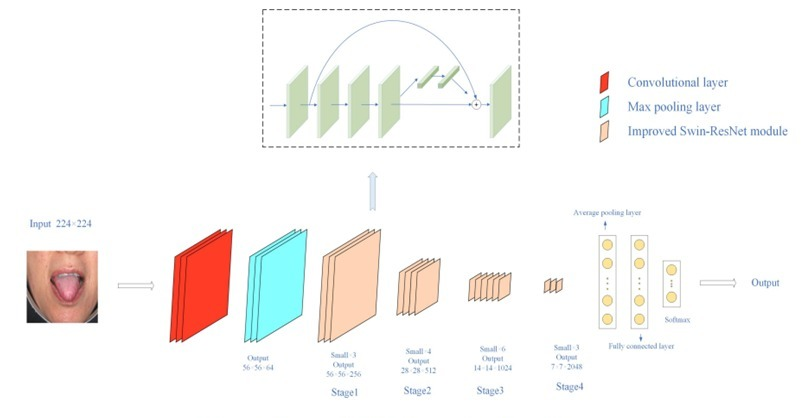
\includegraphics[width=0.80\textwidth]{2/figures/1.jpeg}
		\caption[Metodologia ResNet-50 and Swin Transformer]{Metodologia ResNet-50 and Swin Transformer. \\
		Fuente: \cite{Zhao2024}. \textit{Swin-ResNet: Research and Implementation of a Tooth-Marked
		Tongue Classification Method Combining ResNet-50 and Swin Transformer.}.}
		\label{2:fig123}
	\end{center}
\end{figure}

\cite{Tang2020} desarrollaron un enfoque innovador basado en aprendizaje profundo para la detección automática de lenguas con marcas de dientes, un elemento crucial en el diagnóstico dentro de la medicina tradicional china. El reto principal en este campo radica en la variabilidad de las características visibles de la lengua, particularmente en las marcas dejadas por los dientes en los bordes de la lengua, lo que requiere una metodología de clasificación altamente detallada y precisa. Para abordar este desafío, el equipo implementó una red neuronal convolucional en cascada, compuesta por tres etapas: coarse-Net, fine-Net y refine-Net, que trabajan conjuntamente para detectar y localizar la región de la lengua y los puntos de referencia clave asociados a las marcas dentales. Posteriormente, se emplearon redes ResNet-50 y VGG-16 para llevar a cabo una clasificación precisa de las imágenes de la lengua.

El conjunto de datos utilizado para entrenar y validar este modelo incluyó un total de 1,858 imágenes de lenguas, obtenidas del Hospital Afiliado de la Universidad de Medicina Tradicional China de Chengdu. La implementación de este sistema de aprendizaje profundo mostró una mejora significativa en las métricas de evaluación, superando los enfoques tradicionales que no emplean aprendizaje profundo en cuanto a precisión y consistencia con la percepción humana. El F1-score, que es una medida clave en la evaluación de modelos de clasificación, alcanzó un valor de 0.924 al utilizar ResNet-50, y mejoró aún más a 0.948 cuando se utilizó VGG-16. Estos resultados demostraron que la inclusión de la localización de la región de la lengua y los puntos de referencia de la lengua mejoró significativamente la precisión del modelo.

Este trabajo no solo resalta el potencial del aprendizaje profundo en el ámbito de la medicina tradicional china, sino que también establece un nuevo estándar en la clasificación de lenguas con marcas dentales, destacándose por su capacidad para realizar diagnósticos más rápidos y precisos que los métodos convencionales. La propuesta de \cite{Tang2020} representa un avance pionero en la integración de tecnologías avanzadas de reconocimiento visual para la mejora de diagnósticos médicos en este campo.

La metodología que se empleó para este trabajo fue la siguiente y se puede observar en la Figura \ref{2:fig124}.

\begin{figure}[H]
	\begin{center}
		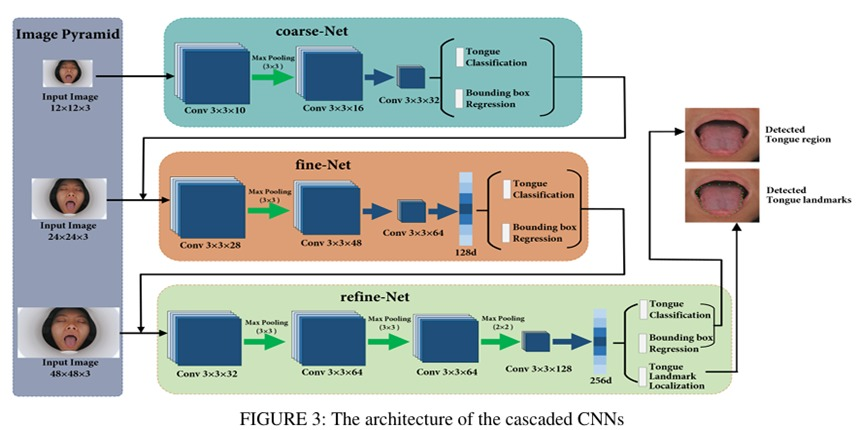
\includegraphics[width=0.80\textwidth]{2/figures/2.jpeg}
		\caption[Metodología ResNet-50 y VGG-16]{Metodología ResNet-50 y VGG-16. \\
		Fuente: \cite{Tang2020}. \textit{An Automatic Recognition of Tooth-Marked Tongue Based on Tongue Region Detection and Tongue Landmark Detection via Deep Learning.}.}
		\label{2:fig124}
	\end{center}
\end{figure}

La investigación llevada a cabo por \cite{Jiatuo2024} aborda el uso de algoritmos de aprendizaje profundo en el análisis y diagnóstico de imágenes de la lengua, un campo crucial en la medicina tradicional china (TCM). Este estudio se centra en el empleo del dataset público BioHit, que contiene 300 imágenes clínicas de lenguas, como base para la experimentación. A través del uso de redes neuronales convolucionales (CNNs) y técnicas de aprendizaje clásico, los autores lograron establecer un marco analítico que combina segmentación, detección de lesiones y clasificación automática de características presentes en las imágenes de lengua.  

En cuanto a la metodología, los investigadores implementaron una red neuronal profunda basada en CNN para extraer características específicas de las imágenes, enfocándose en patrones distintivos como marcas dentales, irregularidades en la textura y variaciones en el revestimiento de la lengua. Este enfoque permitió no solo identificar lesiones con precisión, sino también segmentar regiones clave de interés dentro de las imágenes. Paralelamente, se exploraron modelos clásicos para contrastar los resultados obtenidos con las técnicas más avanzadas.

El estudio reportó resultados significativos al comparar los enfoques clásicos con los de aprendizaje profundo. Mientras que los métodos convencionales alcanzaron una precisión aproximada del 80\% en la detección de lenguas marcadas por dientes, los modelos de aprendizaje profundo lograron precisiones mucho más altas, variando entre el 88\% y el 98.94\%. Entre los modelos más destacados se encuentran ResNet34, con una precisión máxima de 91.47\%, y una red neuronal convolucional multitarea, que alcanzó una precisión sobresaliente del 98.94\%. Este trabajo resalta cómo las técnicas basadas en inteligencia artificial no solo superan a los métodos tradicionales, sino que también aportan un nivel de estandarización y precisión nunca antes visto en el diagnóstico visual en TCM, abriendo nuevas posibilidades para el uso clínico de estas tecnologías.

La metodología seguida en este trabajo puede observarse en la Figura \ref{2:fig125}, la cual resume el proceso desde la segmentación inicial hasta la clasificación final basada en redes neuronales profundas.

\begin{figure}[H]
	\begin{center}
		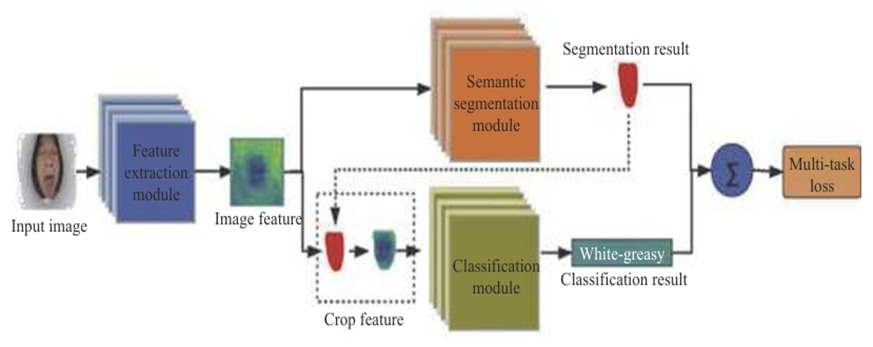
\includegraphics[width=0.80\textwidth]{2/figures/3.jpeg}
		\caption[Metodología de análisis de imágenes de lengua con CNNs]{Metodología de análisis de imágenes de lengua con CNNs. \\
		Fuente: \cite{Jiatuo2024}. \textit{Research status and prospect of tongue image diagnosis analysis based on machine learning.}.}
		\label{2:fig125}
	\end{center}
\end{figure}

En el trabajo de \cite{Liu2023}, se presenta un análisis exhaustivo sobre el uso de la inteligencia artificial en el diagnóstico médico mediante imágenes de lengua, un área relevante en la medicina tradicional china (TCM). A través de una revisión de los estudios más recientes publicados en bases de datos científicas como Web of Science y IEEE en los últimos cinco años, los autores destacan la evolución y los resultados prometedores obtenidos mediante la aplicación de algoritmos de aprendizaje profundo y técnicas híbridas. Este enfoque ha permitido avances significativos en la segmentación, detección y clasificación de imágenes de lengua, optimizando su uso en la diferenciación de síndromes y el diagnóstico de enfermedades.  

La metodología empleada se basa principalmente en el uso de redes neuronales convolucionales (CNNs) y modelos híbridos que integran inteligencia artificial con principios de TCM. Los modelos investigados incluyen técnicas avanzadas como ResNet50 y XGBT optimizado, los cuales se utilizaron para tareas específicas como la calibración y segmentación precisa de regiones de interés en las imágenes de lengua. Además, se destaca la implementación de modelos multitarea, como U-Net, que mejoraron significativamente la capacidad de detección y clasificación de lesiones, incrementando la eficiencia del diagnóstico.  

En términos de resultados, los modelos de aprendizaje profundo lograron precisiones que oscilan entre el 85\% y el 98\% en segmentación y clasificación de enfermedades a partir de imágenes de lengua. Por ejemplo, ResNet50 mostró una precisión de hasta el 92\% en la identificación de condiciones como prediabetes y diabetes. Por otro lado, los modelos híbridos, como un XGBT optimizado, alcanzaron un rendimiento máximo de 98\%, superando a métodos tradicionales en múltiples aspectos. Estas cifras resaltan la capacidad de la inteligencia artificial para transformar el diagnóstico médico al ofrecer mayor precisión y consistencia en los análisis visuales.

Pese a estos avances, los autores también subrayan desafíos importantes que persisten en esta área. Entre ellos se encuentran la necesidad de construir conjuntos de datos más completos y diversos, así como garantizar la fiabilidad en la evaluación de resultados. Además, se menciona que las futuras investigaciones deberían enfocarse en métodos de auto-supervisión y la fusión multimodal de datos, que permitirían una integración más robusta y precisa de la inteligencia artificial en los procesos de diagnóstico médico. Este trabajo establece una base sólida para el desarrollo continuo de tecnologías de diagnóstico inteligente basadas en imágenes de lengua, alineando la medicina tradicional con herramientas modernas de análisis.  

La metodología analizada en este estudio se ilustra en la Figura \ref{2:fig126}, la cual detalla el flujo de trabajo desde la segmentación inicial hasta la clasificación utilizando redes neuronales y modelos híbridos.

\begin{figure}[H]
	\begin{center}
		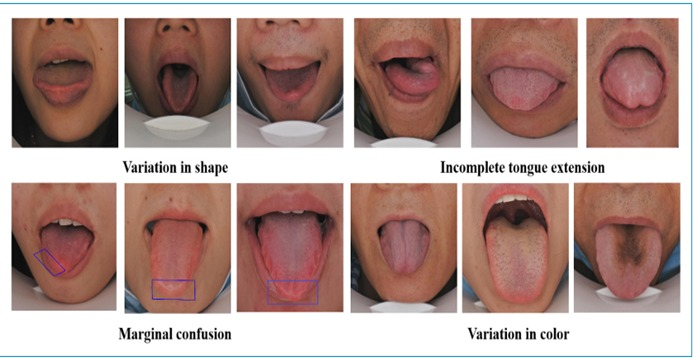
\includegraphics[width=0.80\textwidth]{2/figures/4.jpeg}
		\caption[Enfoque metodológico en el análisis de imágenes de lengua]{Enfoque metodológico en el análisis de imágenes de lengua utilizando modelos híbridos. \\
		Fuente: \cite{Liu2023}. \textit{A survey of artificial intelligence in tongue image for disease diagnosis and syndrome differentiation.}.}
		\label{2:fig126}
	\end{center}
\end{figure}

El estudio realizado por \cite{Jiang2022} examina la aplicación de algoritmos de aprendizaje profundo para el análisis de imágenes de lengua, integrando conocimientos de la medicina tradicional china (TCM). Con un conjunto de datos compuesto por 8,676 imágenes, estas fueron clasificadas en siete categorías distintas: lengua fisurada, marcada por dientes, estasis, con manchas, recubrimiento graso, pelada y podrida. Estas imágenes fueron recopiladas y anotadas por expertos en TCM, lo que garantiza la precisión y relevancia de los datos utilizados.  

La metodología principal implementada en este estudio se basa en el modelo Faster R-CNN, combinado con ResNet101 como extractor de características. Este enfoque permitió la detección y clasificación multietiqueta de las imágenes de lengua con un alto nivel de detalle. Para entrenar el modelo, las imágenes se dividieron en conjuntos de entrenamiento, validación y prueba, y se ejecutaron en un entorno optimizado con GPUs para acelerar los procesos de cálculo. Esta configuración permitió identificar patrones específicos en las imágenes, vinculándolos con características fisiológicas relevantes.  

En cuanto a los resultados, el modelo logró un desempeño destacado, alcanzando una precisión promedio del 90.67\%, una precisión puntual del 99.28\%, un recall del 91.25\% y un F1-score del 95.00\%. Estos indicadores destacan la capacidad del modelo para identificar con precisión características complejas y relevantes en las imágenes de lengua. Además, en una aplicación diagnóstica más amplia, el modelo identificó características específicas en una población de análisis, como lenguas fisuradas (41.49\%), marcadas por dientes (37.16%) y con recubrimiento graso (29.66\%).  

Más allá de la clasificación precisa, el estudio reveló asociaciones significativas entre las características de la lengua y ciertas condiciones metabólicas, como hipertensión, sobrepeso y enfermedades relacionadas con el hígado graso no alcohólico (NAFLD). Estas correlaciones sugieren que las características visibles de la lengua pueden ser indicadores valiosos para diagnósticos tempranos en diversas enfermedades. Asimismo, se identificaron variaciones en la prevalencia de estas características según el género y la edad de los individuos, lo que subraya la importancia de personalizar los análisis diagnósticos.  

\begin{figure}[H]
	\begin{center}
		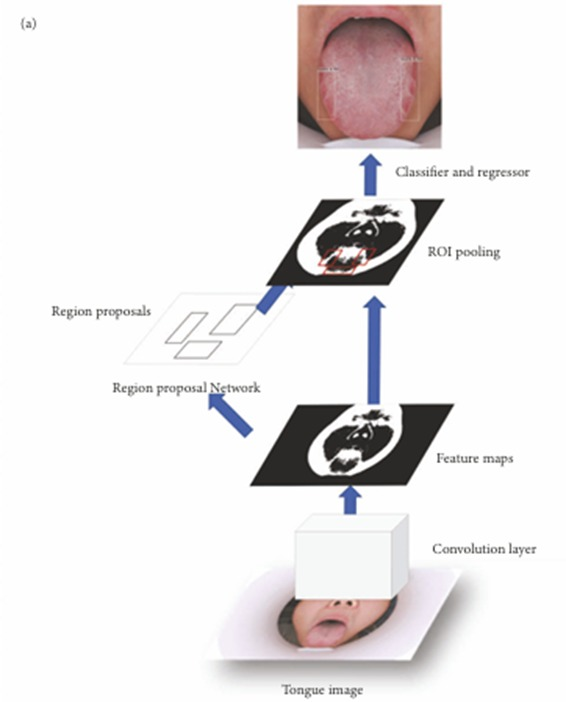
\includegraphics[width=0.7\textwidth]{2/figures/5.jpeg}
		\caption[Metodología con Faster R-CNN y ResNet101]{Metodología con Faster R-CNN y ResNet101 para el análisis de imágenes de lengua. \\
		Fuente: \cite{Jiang2022}. \textit{Deep learning analysis of tongue images in traditional Chinese medicine diagnosis.}.}
		\label{2:fig127}
	\end{center}
\end{figure}

El estudio presentado por \cite{Feasibility2020} analiza la viabilidad de Google’s Teachable Machine (versión 2.0) como herramienta de aprendizaje automático para el diagnóstico de lenguas marcadas por dientes, una característica comúnmente asociada con diversas afecciones de salud bucal. Utilizando un conjunto de datos de 1,250 imágenes obtenidas de Kaggle, el estudio incluye 704 imágenes de lenguas con marcas de dientes y 546 sin marcas, recopiladas y etiquetadas para garantizar su adecuación en aplicaciones diagnósticas.

La metodología se centró en optimizar el rendimiento del modelo ajustando hiperparámetros clave como el número de épocas, el tamaño del lote y la tasa de aprendizaje. El conjunto de datos se dividió en un 90\% para entrenamiento y un 10\% para pruebas, asegurando un adecuado equilibrio entre generalización y precisión. Google’s Teachable Machine, diseñada para simplificar la implementación de modelos de aprendizaje automático, fue utilizada como herramienta base, demostrando que su interfaz accesible puede integrarse en flujos de trabajo clínicos para diagnóstico.

Los resultados obtenidos muestran que el modelo logró una precisión del 92.1\% en la identificación de lenguas marcadas por dientes, mientras que para lenguas sin marcas alcanzó un 72.6\%. La sensibilidad del modelo fue de 0.92, destacando su capacidad para detectar correctamente casos positivos, aunque la especificidad fue baja (0.28), indicando limitaciones en la identificación de casos negativos. Este rendimiento supera al de estudios previos basados en redes neuronales convolucionales más complejas, lo que subraya la efectividad de herramientas accesibles como Teachable Machine en contextos clínicos.

Estos hallazgos no solo resaltan la capacidad de esta herramienta para realizar diagnósticos con una precisión competitiva, sino que también abren la puerta a nuevas aplicaciones en entornos con recursos limitados, donde el acceso a infraestructura avanzada de aprendizaje profundo es restringido. Además, el enfoque simplificado de Google’s Teachable Machine facilita la adopción de tecnologías de inteligencia artificial en la práctica médica, permitiendo a los profesionales implementar soluciones rápidas y eficientes para el diagnóstico de condiciones clínicas.

\begin{figure}[H]
	\begin{center}
		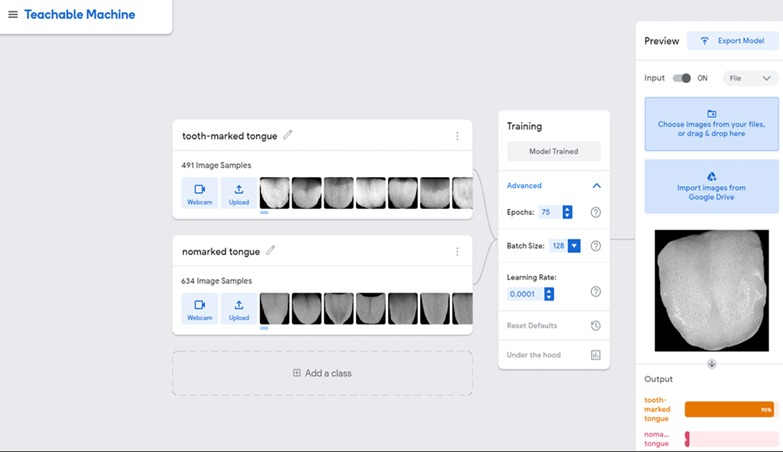
\includegraphics[width=0.80\textwidth]{2/figures/6.jpeg}
		\caption[Flujo de trabajo en Google’s Teachable Machine]{Flujo de trabajo para diagnóstico de lengua marcada por dientes utilizando Google’s Teachable Machine. \\
		Fuente: \cite{Feasibility2020}. \textit{Feasibility Study of Google's Teachable Machine in Diagnosis of Tooth-Marked Tongue.}.}
		\label{2:fig128}
	\end{center}
\end{figure}

El estudio de \cite{Kong2020} presenta una metodología avanzada para la detección y análisis de lenguas marcadas por dientes, un rasgo distintivo en el diagnóstico de la medicina tradicional china (TCM), que puede estar asociado con disfunciones en órganos internos como el hígado y el bazo. Este trabajo se basa en un conjunto de datos compuesto por 1,500 imágenes clínicas de alta calidad provenientes del Hospital Shu Guang en Shanghái. Dentro de este conjunto, se seleccionaron específicamente 400 imágenes de lenguas normales y 756 con marcas de dientes, las cuales fueron etiquetadas manualmente para garantizar la precisión en la segmentación y localización de las marcas.

La metodología empleada combina el poder del modelo Mask Scoring R-CNN con técnicas de aprendizaje por transferencia, utilizando ResNet-101 como red base. Este enfoque permitió una segmentación precisa y una localización detallada de las marcas dentales presentes en las imágenes. Antes del entrenamiento del modelo, las imágenes fueron sometidas a un proceso de preprocesamiento intensivo, incluyendo la normalización del color, recorte y etiquetado manual de las áreas de interés para generar máscaras altamente detalladas. Estos pasos fueron fundamentales para optimizar la detección de marcas dentales, especialmente en casos con grados de severidad diversos.

Los resultados del estudio fueron sobresalientes. El modelo alcanzó un F1-score de 0.95, lo que refleja un equilibrio casi perfecto entre precisión y recall. Además, la precisión específica del modelo fue del 99\%, mientras que el recall alcanzó un valor notable de 91.4\%. Estos indicadores demuestran no solo la alta precisión del modelo, sino también su capacidad para generalizar en diferentes escenarios clínicos. Esto es particularmente relevante dado que las lenguas marcadas por dientes pueden variar significativamente en términos de su apariencia y severidad.

Una de las contribuciones más destacadas de esta investigación es su aplicabilidad en el ámbito de la telemedicina. Al integrar herramientas avanzadas de aprendizaje profundo como Mask Scoring R-CNN, se abre la posibilidad de realizar diagnósticos detallados a distancia, reduciendo la dependencia de evaluaciones presenciales y facilitando el acceso a servicios médicos especializados. Esto es especialmente relevante en áreas donde la medicina tradicional china es una práctica común, pero los recursos médicos pueden ser limitados.

\begin{figure}[H]
	\begin{center}
		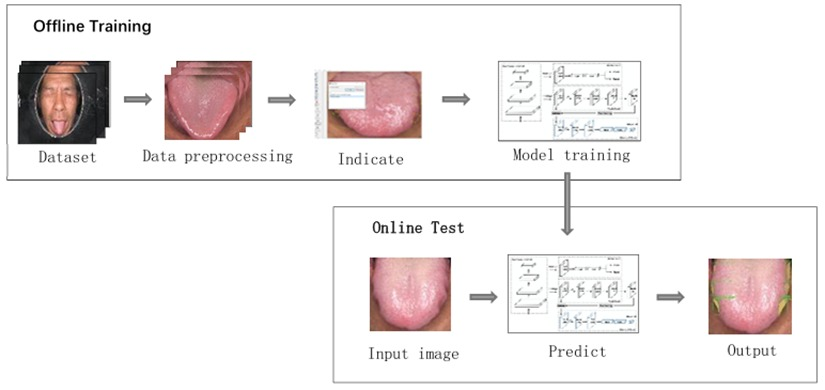
\includegraphics[width=0.80\textwidth]{2/figures/7.jpeg}
		\caption[Detección de lengua marcada por dientes con Mask Scoring R-CNN]{Esquema de segmentación y localización de marcas dentales utilizando Mask Scoring R-CNN con ResNet-101. \\
		Fuente: \cite{Kong2020}. \textit{Tooth-marked tongue recognition based on Mask Scoring R-CNN.}}
		\label{2:fig129}
	\end{center}
\end{figure}

Este estudio subraya la relevancia de la inteligencia artificial en la modernización de los diagnósticos basados en imágenes, mostrando cómo modelos avanzados pueden superar las limitaciones tradicionales de precisión y consistencia en el análisis de características complejas como las marcas de dientes en la lengua.

El trabajo de \cite{Tiryaki2024} explora el uso de redes neuronales profundas (DCNN) en la identificación y clasificación de lesiones en la lengua, un campo emergente con importantes aplicaciones clínicas. Este estudio aborda específicamente cinco categorías: lengua normal y cuatro tipos de lesiones comunes, incluyendo lengua fisurada, lengua geográfica, lengua recubierta y glositis romboidal mediana. Para este análisis, se recopiló un conjunto de datos compuesto por 623 imágenes clínicas de lengua, etiquetadas de manera experta para garantizar la precisión en la categorización.

La metodología implementada incluyó el uso de varios modelos avanzados de DCNN, como VGG19, ResNet50, ResNet101 y GoogLeNet. Estos modelos se beneficiaron del aprendizaje por transferencia, una técnica que aprovecha redes preentrenadas para mejorar la eficiencia en problemas con datos limitados. Además, este estudio introdujo por primera vez en este contexto un enfoque innovador basado en la fusión por votación mayoritaria (FBMV, por sus siglas en inglés), diseñado para combinar las predicciones de múltiples modelos y mejorar la precisión global.

Los resultados obtenidos fueron notables tanto en la clasificación binaria como en la clasificación multiclase. En la tarea binaria (lengua normal vs. lengua con lesiones), el modelo ResNet101 logró una precisión inicial del 93.53\%. Este rendimiento fue mejorado significativamente mediante la aplicación del enfoque FBMV, alcanzando un 95.15\%. Para la clasificación multiclase, que abarcó las cinco categorías, VGG19 se destacó con una precisión del 83.93\%, la cual fue incrementada al 88.76\% tras incorporar FBMV. Estos resultados no solo demuestran la robustez de las redes neuronales profundas en la detección de características complejas de la lengua, sino también el valor añadido del enfoque de fusión para abordar problemas de clasificación con múltiples clases.

Además de los resultados cuantitativos, el estudio subraya el potencial de estas tecnologías en el ámbito clínico. La capacidad de las DCNN para identificar patrones sutiles y correlaciones en imágenes médicas abre nuevas posibilidades para diagnósticos automatizados y personalizados. Este avance es especialmente relevante en entornos con recursos limitados, donde las herramientas basadas en inteligencia artificial pueden complementar la experiencia de los profesionales de la salud, mejorando la eficiencia y reduciendo los tiempos de diagnóstico.

\begin{figure}[H]
	\begin{center}
		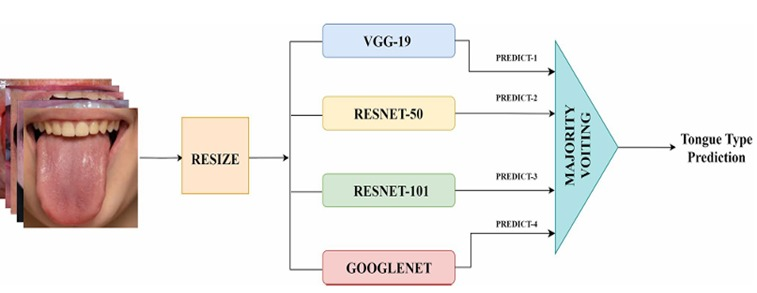
\includegraphics[width=0.85\textwidth]{2/figures/8.jpeg}
		\caption[Clasificación de lesiones linguales con DCNN y FBMV]{Estrategia de fusión por votación mayoritaria aplicada a modelos DCNN para clasificaciones binaria y multiclase. \\
		Fuente: \cite{Tiryaki2024}. \textit{Artificial intelligence in tongue diagnosis: classification of tongue lesions and normal tongue images using deep convolutional neural network.}}
		\label{2:fig130}
	\end{center}
\end{figure}

En conclusión, este trabajo destaca cómo la integración de DCNN y enfoques innovadores como FBMV puede transformar el diagnóstico de enfermedades bucales, proporcionando una base sólida para investigaciones futuras y desarrollos tecnológicos en medicina basada en imágenes.


\section{Bases Teóricas}
\subsection{Bruxismo en niños}

\subsubsection{Definición}

El término "bruxismo" proviene del griego "brygmós", que significa "apretar o rechinar los dientes". Este trastorno, también conocido como la "enfermedad silenciosa", afecta aproximadamente al 70\% de los pacientes, y su aparición se vincula principalmente al estrés y problemas psicológicos \parencite{Rojas2022}. Según lo descrito por \textcite{Rojas2022}, el bruxismo representa un desafío común en la salud dental a nivel mundial, generando alteraciones en el aparato masticatorio y contribuyendo a cambios morfológicos que comprometen la salud bucal.

Es importante destacar que el término "bruxismo" suele confundirse con otros relacionados, como bruxismo céntrico, excéntrico, nocturno, diurno, bruxomanía, parafunción, apretamiento dentario, rechinamiento dentario, entre otros \parencite{Zambra2003}.

\subsubsection{Síntomas}

Los síntomas del bruxismo en niños incluyen sonidos audibles durante el acto de apretar o rechinar los dientes, ya sea consciente o inconscientemente. Estos pueden manifestarse como chasquidos o movimientos dentales en posición céntrica o excéntrica, durante actividades como la deglución o masticación, tanto de día como de noche \parencite{vallejo2002bruxismoinfantil}. 

La magnitud de los síntomas depende de la resistencia de las estructuras involucradas y de factores como la duración, frecuencia e intensidad del bruxismo. Aunque algunas estructuras del sistema masticatorio absorben estas fuerzas sin consecuencias, otras experimentan daños que van desde el desgaste dental hasta alteraciones en los músculos masticatorios y las articulaciones temporomandibulares \parencite{vallejo2002bruxismoinfantil}.

\subsubsection{Factores de riesgo}

\paragraph{Factores odontológicos}  
El bruxismo puede estar influido por condiciones como maloclusiones esqueléticas, alteraciones oclusales y restauraciones dentales defectuosas. Sin embargo, los estudios en este ámbito han arrojado resultados inconsistentes \parencite{Zambra2003}.

\paragraph{Factores psicológicos}  
El estrés y la ansiedad son factores psicológicos clave asociados al bruxismo, especialmente en adolescentes. Un estudio indicó que los niveles elevados de catecolaminas en la orina de niños de 6 a 8 años podrían estar relacionados con altos niveles de ansiedad \parencite{vanderas1999catecholaminebruxism}. Sin embargo, otros factores como el nivel socioeconómico y cultural no muestran resultados concluyentes \parencite{serranegra2009psychosocialbruxism}.

\paragraph{Factores relacionados con el sueño}  
El bruxismo nocturno, considerado una parasomnia, ocurre durante el sueño y está relacionado con despertares parciales y altos niveles de estrés emocional. Aunque estas alteraciones son comunes en la infancia, su frecuencia persistente puede indicar problemas psicológicos subyacentes \parencite{vieiraandrade2014sleepbruxism}.

\paragraph{Factores genéticos}  
Evidencia sugiere que el bruxismo puede tener una base genética, ya que los niños cuyos padres presentaron bruxismo tienen mayor probabilidad de desarrollarlo, lo que señala una predisposición hereditaria \parencite{hublin2001parasomniasgenetics}.

\subsection{Diagnóstico y prediagnóstico del bruxismo}

\subsubsection{Método instrumental}  
La polisomnografía es considerada la técnica de referencia para diagnosticar el bruxismo durante el sueño, ya que permite un monitoreo completo de la actividad cerebral, muscular y respiratoria. Asimismo, los registros electromiográficos (EMG) y las aplicaciones móviles emergen como herramientas innovadoras para evaluar la actividad muscular en tiempo real \parencite{gutierrez2021bruxismorino}.

\subsubsection{Método no instrumental}  
El diagnóstico mediante autorreporte y evaluación clínica es ampliamente utilizado debido a su accesibilidad y bajo costo. Sin embargo, estos métodos presentan limitaciones en comparación con los instrumentales, por lo que su precisión aún debe ser mejorada \parencite{gutierrez2021bruxismorino}.

\subsection{Aprendizaje profundo y visión por computadora}

\subsubsection{Definición}  
El aprendizaje profundo, según \textcite{kim2017matlabdeeplearning}, se basa en redes neuronales con múltiples capas ocultas. Estas estructuras permiten procesar datos complejos de manera jerárquica, lo que constituye la esencia del Deep Learning.

\subsubsection{Visión por computadora}  
La visión por computadora busca replicar la capacidad humana de interpretar información visual a través de algoritmos y modelos matemáticos. Este campo, iniciado por David Marr en la década de 1980, ha evolucionado hacia aplicaciones que abarcan desde la robótica hasta el diagnóstico médico \parencite{szeliski2010computervision}.

\subsubsection{Aplicación en la salud}  
En medicina, la visión por computadora permite detectar patrones y anomalías en imágenes médicas como radiografías y resonancias magnéticas. Por ejemplo, las redes neuronales convolucionales han demostrado ser eficaces en la identificación de tumores, mejorando la velocidad y precisión del diagnóstico \parencite{litjens2017deeplearningmedical}.

\subsection{Aplicaciones móviles}

\subsubsection{Definición}  
Las aplicaciones móviles son programas diseñados para dispositivos como smartphones y tablets, ofreciendo una amplia gama de funcionalidades que van desde el entretenimiento hasta la salud \parencite{marinescu2019mobileappdev}.

\subsubsection{Importancia en la salud}  
Estas aplicaciones han revolucionado la gestión de la salud al ofrecer herramientas personalizadas para el monitoreo, la consulta y la toma de decisiones informadas. Además, promueven la autonomía de los pacientes al proporcionar acceso inmediato a información confiable \parencite{marinescu2019mobileappdev}.


\section{Marco Conceptual}
\subsection{Bruxismo primario}
El bruxismo primario, también conocido como idiopático, es un trastorno caracterizado por el hábito inconsciente de apretar o rechinar los dientes, especialmente durante el sueño. A diferencia del bruxismo secundario, no se asocia a una causa médica o psicológica identificable. Se cree que factores genéticos, estrés y trastornos del sueño podrían estar involucrados en su desarrollo. A largo plazo, el bruxismo primario puede causar desgaste dental, dolor en la mandíbula y otros problemas bucales \parencite{kato2001epidemiologybruxism}.

\subsection{Disfunción temporomandibular}
La disfunción temporomandibular (DTM) se caracteriza por diversos síntomas, incluyendo dolor en la región bucal, sonidos en las articulaciones y restricciones en los movimientos de la mandíbula. Esta condición tiene múltiples causas, que abarcan desde traumatismos y hábitos parafuncionales hasta el estrés, todos los cuales pueden exceder la capacidad fisiológica de los individuos. Factores como la estabilidad articular, la oclusión dental y características genéticas también son determinantes. Un estudio indica que hay una relación entre el bruxismo durante el sueño y la presencia de dolor en pacientes con DTM, lo que enfatiza la necesidad de una evaluación exhaustiva para su tratamiento \parencite{blanco2014selfreportbruxism}.

\subsection{Cefaleas}
Las cefaleas son uno de los trastornos más frecuentes del sistema nervioso, afectando a aproximadamente la mitad de los adultos en el último año y siendo la sexta causa de incapacidad en el mundo. Aunque la mayoría no son graves, es importante buscar atención médica si el dolor es intenso y repentino, o si se acompaña de síntomas neurológicos o fiebre \parencite{clinica2018cefalea}.

\subsection{Sensibilidad dental}
La hipersensibilidad dentinaria (HD), también conocida como sensibilidad dental, se caracteriza por un dolor intenso y temporal en los dientes, que ocurre debido a la exposición de la dentina al entorno bucal. Este tipo de dolor se desencadena por estímulos externos como alimentos o bebidas frías, calientes, ácidas o dulces, así como por la presión táctil \parencite{dentaid2024sensibilidad}.

\subsection{Odontología del sueño}
La medicina dental del sueño es una especialidad odontológica que se ocupa del tratamiento de los trastornos del sueño, siendo el síndrome de apnea obstructiva del sueño (SAOS) y los ronquidos las afecciones más comunes tratadas \parencite{gutierrez2021bruxismorino}.

\subsection{Lingua geográfica}
La lengua geográfica es una condición inflamatoria que, aunque no representa un riesgo, se manifiesta en la superficie de la lengua. En esta afección, la lengua presenta pequeñas protuberancias de color blanco rosado, conocidas como papilas, que son estructuras finas similares a vellos. En las áreas afectadas por la lengua geográfica, las papilas están ausentes, dejando zonas suaves y rojas, a menudo con bordes ligeramente elevados \parencite{mayoclinic2024lenguageografica}.

\subsection{Redes neuronales convolucionales}
\subsubsection{Definición y funcionamiento}
Las redes neuronales convolucionales (CNN) son un tipo de red neuronal organizadas en varias capas, conocidas como multicapa. Estas redes presentan una arquitectura donde las neuronas están interconectadas. 

\subsubsection{Componentes principales}
Se componen de una capa de convolución, donde cada neurona filtra la información de entrada para generar un mapa de características; seguida por una capa de submuestreo, que reduce el tamaño de la información procesada; y finalmente, una capa completamente conectada que se encarga de la clasificación. Las CNN son especialmente eficaces en proyectos de procesamiento de imágenes gracias a su capacidad de clasificación \parencite{lopezpacheco2021redesconv}.

\subsection{Support Vector Machines (SVM)}
Las Support Vector Machines son un conjunto de métodos de aprendizaje supervisado utilizados para clasificación y regresión. Se basan en encontrar un hiperplano óptimo que separa diferentes clases en un espacio multidimensional. Este hiperplano maximiza el margen entre las clases más cercanas, llamadas vectores de soporte. Las SVM son efectivas en espacios de alta dimensión y pueden utilizarse con distintos tipos de núcleos (kernels) para manejar problemas no lineales \parencite{cortes1995svm}.

\subsection{Extracción de características}
La extracción de características es el proceso de transformar datos en bruto y complejos en representaciones numéricas más simples y significativas, llamadas características. Estas características son luego utilizadas como entrada para algoritmos de aprendizaje automático, permitiendo a las máquinas "entender" y aprender de los datos \parencite{szeliski2010computervision}.

\subsection{Transfer learning}
El \textit{transfer learning} permite utilizar modelos preentrenados en un nuevo conjunto de datos, facilitando la mejora del rendimiento cuando se dispone de pocos datos. Esto ahorra tiempo y recursos durante el entrenamiento, aprovechando el conocimiento previo \parencite{pan2010survey}.

\subsection{Data augmentation}
El \textit{data augmentation} amplía un conjunto de datos mediante transformaciones como rotaciones y escalados. Esta técnica mejora la robustez del modelo y reduce el riesgo de sobreajuste, creando un conjunto más diverso para el entrenamiento \parencite{shorten2019survey}.

\subsection{Segmentación de imágenes}
La segmentación de imágenes divide una imagen en regiones significativas para facilitar la identificación de objetos. Es esencial en tareas de detección y reconocimiento, utilizando redes neuronales para lograr alta precisión \parencite{litjens2017deeplearningmedical}.

\subsection{Redes generativas adversarias}
Las redes generativas adversarias (GANs) consisten en un generador y un discriminador que compiten entre sí. El generador crea datos sintéticos, mientras que el discriminador evalúa su autenticidad. Son efectivas en la generación de imágenes y la mejora de resolución \parencite{goodfellow2014generative}.

\subsection{Pooling}
El \textit{pooling} es una técnica utilizada en redes neuronales convolucionales (CNN) para reducir la dimensionalidad de los mapas de características generados por las capas de convolución. Este proceso consiste en aplicar una función de agregación, como la máxima (\textit{max pooling}) o la media (\textit{average pooling}), sobre bloques de características. Ayuda a disminuir la carga computacional, mejora la generalización del modelo y hace que las redes sean menos sensibles a pequeñas variaciones en la entrada \parencite{boureau2010theoretical}.

\subsection{Regularización}
La regularización previene el sobreajuste en modelos de aprendizaje automático. Incluye técnicas como la penalización de coeficientes y el \textit{dropout}, que apaga neuronas aleatoriamente durante el entrenamiento para mejorar la generalización del modelo \parencite{srivastava2014dropout}.


\section{Hipótesis}
\subsection{Hipótesis General}
HG: \newcommand{\HipotesisGeneral}{
	El uso de un sistema automatizado basado en técnicas de aprendizaje profundo, como las redes neuronales convolucionales (CNN), permite realizar un prediagnóstico efectivo del bruxismo en niños mediante la identificación de patrones visuales en imágenes de la lengua, con una precisión comparable o superior a los métodos diagnósticos tradicionales.
	}
\HipotesisGeneral


\subsection{Hipótesis Específicas}
\newcommand{\Hone}{
	Un modelo de aprendizaje profundo, específicamente una red neuronal convolucional (CNN), puede clasificar imágenes de la lengua con alta precisión para detectar signos de bruxismo en niños.
	}
\newcommand{\Htwo}{
	Existen patrones visuales distintivos en las imágenes de la lengua que están relacionados con episodios de bruxismo en niños.
	}
\newcommand{\Hthree}{
	Las técnicas de procesamiento de imágenes, como la segmentación y el análisis de texturas, son efectivas para extraer características relevantes de las imágenes de la lengua para el diagnóstico de bruxismo.
	}
\newcommand{\Hfour}{
	El sistema automatizado basado en aprendizaje profundo logra una precisión, sensibilidad y especificidad competitivas en la detección de bruxismo en niños en comparación con los métodos tradicionales.
	}
\newcommand{\Hfive}{
	La implementación de un sistema automatizado para el análisis de imágenes de la lengua incrementa la tasa de detección temprana de bruxismo en niños, facilitando su diagnóstico en entornos clínicos y domésticos.
		}

\begin{itemize}
	\item HE1: {\Hone}
	\item HE2: {\Htwo}
	\item HE3: {\Hthree}
	\item HE4: {\Hfour}
	\item HE5: {\Hfive}
\end{itemize}

%\chapter{Metodología de la Investigación}
\section{Diseño de la investigación}
El diseño de esta investigación es de tipo cuasi-experimental, ya que se observará la relación entre las marcas en los bordes de la lengua (variable independiente) y la presencia de bruxismo (variable dependiente) en niños, sin manipular el entorno ni asignar condiciones al azar. Las imágenes de las lenguas serán procesadas mediante técnicas de visión computacional para extraer características clave, que luego serán evaluadas mediante modelos de deep learning. Este enfoque permite analizar patrones asociados al bruxismo de forma controlada y sistemática, sin alterar las condiciones naturales de los participantes.

\subsection{Alcance de la investigación}
El nivel de esta investigación es explicativo, ya que se busca desarrollar una aplicación móvil que permita el prediagnóstico de bruxismo en niños mediante el análisis de imágenes de sus lenguas. El sistema de visión computacional que se propone está diseñado para identificar patrones específicos, como las marcas en los bordes de la lengua, los cuales podrían estar asociados a esta condición. Este enfoque permite establecer una relación de causa-efecto, donde la presencia de ciertos patrones en las imágenes analizadas puede servir como indicador preliminar de bruxismo, facilitando una detección temprana y preventiva.

\subsection{Enfoque de la investigación}
El enfoque de esta investigación es cuantitativo, ya que se busca obtener datos medibles para el prediagnóstico de bruxismo en niños. Para esto, se emplearán imágenes de lenguas de niños con posibles signos de bruxismo, específicamente marcas en los bordes, que serán procesadas mediante técnicas de visión computacional. Los resultados obtenidos serán datos numéricos que permitirán entrenar modelos de deep learning para identificar patrones asociados al bruxismo. Estos modelos se utilizarán como herramienta de apoyo para el prediagnóstico, aportando precisión y rapidez en la detección de esta condición en una etapa temprana.

\subsection{Población}
La población de esta investigación está constituida por individuos que presentan posibles señales de bruxismo, específicamente aquellos con marcas en los bordes de la lengua identificadas mediante examen visual o imágenes clínicas.

\subsection{Muestra}
La muestra utilizada en esta investigación consiste en un conjunto de 1250 imágenes de lenguas marcadas y no marcadas, obtenidas de la plataforma kaggle, de las cuales todas fueron tomadas de personas con posibles señales de bruxismo.

\section{Operacionalización de variables}
En este apartado se describen las principales variables del estudio, detallando su definición conceptual, definición operacional, los indicadores asociados, así como el instrumento y la escala utilizada para su medición. Estas variables permiten estructurar y guiar el proceso de análisis basado en técnicas de aprendizaje profundo.

\begin{table}[H]
\centering
\caption{Definición de variables del estudio.}
\label{tabla:variables}
\begin{tabular}{|p{2.5cm}|p{3cm}|p{3.5cm}|p{2.5cm}|p{2.5cm}|p{1.5cm}|}
\hline
\textbf{Variable} & \textbf{Definición Conceptual} & \textbf{Definición Operacional} & \textbf{Indicadores} & \textbf{Instrumento} & \textbf{Escala} \\ \hline
\textbf{Marcas en los bordes de la lengua} & Signos visuales en el borde de la lengua indicativos de bruxismo. & Detección de marcas en imágenes procesadas mediante técnicas de visión computacional. & Presencia o ausencia de marcas. & Modelo de \textit{deep learning}. & Nominal \\ \hline
\textbf{Presencia de bruxismo} & Apretamiento o rechinamiento involuntario de dientes, identificado por signos en lengua. & Diagnóstico preliminar basado en patrones visuales asociados al bruxismo. & Predicción del modelo. & Modelo de \textit{deep learning}. & Nominal \\ \hline
\end{tabular}
\end{table}

\section{Técnicas de recolección de datos}
En esta sección se describen las técnicas utilizadas para la obtención y el procesamiento de los datos necesarios para el desarrollo del modelo de aprendizaje profundo. Se detalla la fuente de datos, el proceso de recolección y las herramientas empleadas en el análisis.

\begin{table}[H]
    \caption{Técnicas de recolección de datos.}
    \centering
    \renewcommand{\arraystretch}{1.5} % Aumenta el espacio entre filas
    \setlength{\tabcolsep}{8pt} % Ajusta el espacio entre columnas
    \begin{tabular}{|p{4cm}|p{10cm}|}
        \hline
        \textbf{Técnica} & \textbf{Descripción} \\ \hline
        Fuente de datos & 1250 imágenes de lenguas marcadas y no marcadas obtenidas de Kaggle. \\ \hline
        Proceso de recolección & Selección, preprocesamiento y etiquetado de las imágenes para la detección de marcas indicativas de bruxismo. \\ \hline
        Herramientas utilizadas & Visión computacional para detección de características y \textit{deep learning} para análisis y clasificación de imágenes. \\ \hline
    \end{tabular}
\end{table}


\section{Metodología de Implementación de la Solución}

La metodología propuesta para implementar un modelo de \textit{Deep Learning} está basada en el ciclo de vida de desarrollo de modelos de Inteligencia Artificial, con adaptaciones específicas para abordar el diagnóstico de bruxismo en niños mediante patrones de sonido y frecuencia, así como el análisis de imágenes de lengua.

Para este caso, se busca desarrollar un modelo de \textit{Deep Learning} que asista en el prediagnóstico de bruxismo infantil. La metodología propuesta toma como referencia algunos enfoques presentados en los antecedentes revisados, adaptándolos para el análisis de datos de sonido y procesamiento de imágenes relacionadas con marcas en los bordes de la lengua. En la Figura \ref{3:fig301} se presenta de manera gráfica la metodología propuesta para este proyecto.

\begin{figure}[H]
	\begin{center}
		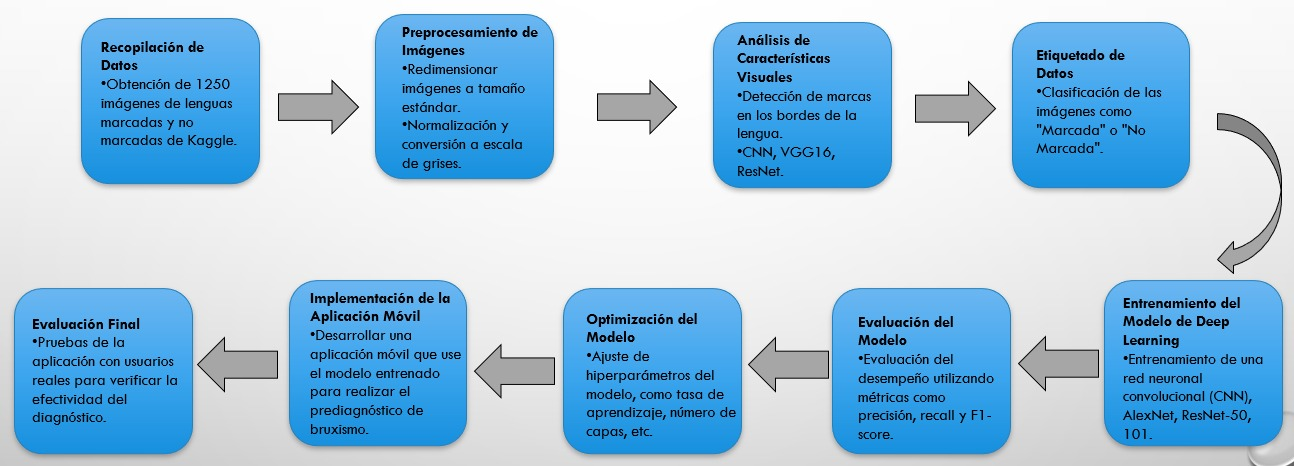
\includegraphics[width=1.00\textwidth]{3/figures/1.jpeg}
		\caption[Metodología de implementación]{Metodología de implementación. \\
		Fuente: Elaboración propia.}
		\label{3:fig301}
	\end{center}
\end{figure}





%\include{4/desarrollo}
%\include{5/resultados}
%\include{6/conclusion}

%%Para insertar los capítulos de forma seguida
\chapter{Planteamiento del Problema}
\section{Descripción de la Realidad Problemática}

El bruxismo, definido como una actividad repetitiva de los músculos mandibulares que incluye el apretamiento o rechinamiento involuntario de los dientes, es una condición muy frecuente en la población infantil. De acuerdo con la Academia Americana de Medicina del Sueño, este hábito no controlado ocurre principalmente durante las horas de descanso nocturno y puede generar importantes repercusiones tanto en la salud bucal como en el bienestar general del niño \parencite{AmericanAcademy2014}.

La prevalencia de esta condición en niños es un tema ampliamente investigado, pero con resultados variables dependiendo de los contextos geográficos y los enfoques metodológicos utilizados en los estudios. Según una revisión sistemática, la prevalencia de bruxismo en niños menores de 12 años puede oscilar entre el 3.5\% y el 40.6\%, sin observarse diferencias significativas en cuanto a género \parencite{Manfredini2013}. En países de América Latina, como Brasil, los estudios indican cifras que varían entre un 32\% y un 43\%, mientras que en Chile se ha reportado una prevalencia cercana al 32\%, con un aumento hasta el 38\% en niños de 6 años \parencite{Shinkai1998, Sandoval2016}.

El bruxismo infantil puede clasificarse en dos categorías principales: bruxismo del sueño y bruxismo de vigilia. Aunque ambos tipos presentan características comunes, el bruxismo del sueño es más prevalente en niños, aunque frecuentemente pasa desapercibido en sus etapas iniciales. Esto dificulta su detección y tratamiento oportunos, incrementando el riesgo de complicaciones a largo plazo \parencite{Camoin2017}.

Diversos estudios destacan la naturaleza multifactorial del bruxismo infantil, identificando factores locales, psicológicos, hereditarios y fisiopatológicos como principales contribuyentes. Por ejemplo, las maloclusiones dentales, el estrés emocional y la ansiedad son factores recurrentes, mientras que una predisposición genética también juega un rol significativo. En particular, investigaciones han evidenciado que los niños cuyos padres tienen antecedentes de bruxismo presentan una mayor probabilidad de desarrollar esta condición \parencite{Abe1966, Lobbezoo1997}.

Una de las mayores dificultades en el diagnóstico del bruxismo en niños radica en distinguir entre el desgaste natural de los dientes asociado al desarrollo y el desgaste patológico provocado por esta condición. Los profesionales de la salud generalmente recurren a cuestionarios dirigidos a los padres para recopilar información, complementándolos con un examen clínico detallado del niño. Sin embargo, en casos más graves, la polisomnografía (PSG) se considera el estándar de oro para registrar los episodios de bruxismo durante el sueño \parencite{Luiz2008, Sandoval2016}. A pesar de su eficacia, la PSG presenta limitaciones significativas, como altos costos, infraestructura compleja y la incomodidad que genera en pacientes pediátricos \parencite{Chisini2020}.

Adicionalmente, estudios recientes han asociado el bruxismo con problemas respiratorios, como la apnea obstructiva del sueño (AOS), en la que los movimientos mandibulares pueden ser intentos del cuerpo para mejorar el flujo de aire durante el sueño \parencite{Bulanda2021, Goettems2017}. Estas conexiones subrayan la necesidad de métodos diagnósticos más accesibles y no invasivos. En este contexto, herramientas tecnológicas basadas en aprendizaje profundo, que analicen patrones como los movimientos mandibulares y las características observables en la lengua, podrían revolucionar la forma en que se diagnostica esta condición \parencite{Chisini2020}.

En Perú, los estudios reflejan cifras preocupantes. En La Brea, Piura, el 65.22\% de los niños entre 4 y 6 años presentan signos de bruxismo, con una mayor incidencia en niños de 5 años \parencite{Baldeon2014}. Asimismo, en Buenos Aires, Piura, se encontró una prevalencia de hasta el 69.8\% en niños preescolares \parencite{Delgado2002}. Estas cifras superan ampliamente las reportadas en países como Estados Unidos, donde la prevalencia alcanza el 38\% \parencite{Cheifetz2005}, o en Brasil, con un 43\% \parencite{Valera2003}.

Aunque factores como las parasitosis intestinales han sido objeto de estudio en relación con el bruxismo en Perú, no se ha hallado una correlación significativa \parencite{Baldeon2014}. Sin embargo, la alta prevalencia de esta condición justifica el desarrollo de soluciones tecnológicas innovadoras, como aplicaciones móviles basadas en aprendizaje profundo, para facilitar un diagnóstico temprano y más preciso.

En conclusión, el bruxismo infantil constituye una condición prevalente con múltiples factores etiológicos. Su diagnóstico oportuno es crucial para prevenir consecuencias graves, como desgaste dental severo, problemas musculares y articulares, así como alteraciones en el desarrollo facial. La implementación de tecnologías accesibles y no invasivas representa un paso adelante en la mejora de la calidad de vida de los niños afectados, al tiempo que permite optimizar los recursos en entornos de atención médica.

\section{Formulación del Problema}
Con el objetivo de formular los objetivos de esta investigación, se propusieron las siguientes preguntas.
\subsection{Problema General}
PG: \newcommand{\ProblemaGeneral}{
	¿Puede un sistema automatizado, basado en técnicas de aprendizaje profundo, realizar un prediagnóstico efectivo del bruxismo en niños mediante la identificación de características en imágenes de la lengua?
}
\ProblemaGeneral
\subsection{Problemas Específicos}
\newcommand{\Pbone}{
	¿Cómo se puede diseñar un modelo de aprendizaje profundo, como redes neuronales convolucionales (CNN), para clasificar imágenes de la lengua y detectar signos de bruxismo?
	}
\newcommand{\Pbtwo}{
	¿Cuáles son los patrones visuales en imágenes de la lengua que están asociados con episodios de bruxismo en niños?
	}
\newcommand{\Pbthree}{
	¿Qué técnicas de procesamiento de imágenes y extracción de características son más efectivas para identificar signos de bruxismo a partir de imágenes de la lengua?
	}
\newcommand{\Pbfour}{
	¿Cuál es la precisión y tasa de éxito del sistema propuesto en comparación con los métodos diagnósticos tradicionales?
	}
\newcommand{\Pbfive}{
	¿Cómo contribuye la implementación de un sistema automatizado basado en el análisis de imágenes al incremento de la detección temprana de bruxismo en niños?
}

\begin{itemize}
	\item PE1: {\Pbone}
	\item PE2: {\Pbtwo}
	\item PE3: {\Pbthree}
	\item PE4: {\Pbfour}
	\item PE5: {\Pbfive}
\end{itemize}

\section{Objetivos de la Investigación}
A continuación, se presentan el objetivo general y los objetivos específicos.
\subsection{Objetivo General}
OG: \newcommand{\ObjetivoGeneral}{
	Desarrollar y validar un sistema automatizado basado en técnicas de aprendizaje profundo para el prediagnóstico de bruxismo en niños, utilizando el análisis de imágenes de la lengua.
	}
\ObjetivoGeneral
\subsection{Objetivos Específicos}
\newcommand{\Objone}{
	Diseñar un modelo de aprendizaje profundo, específicamente una red neuronal convolucional (CNN), que pueda clasificar con precisión las imágenes de la lengua para identificar episodios de bruxismo.
	}
\newcommand{\Objtwo}{
	Identificar y analizar los patrones visuales en imágenes de la lengua que son indicativos de bruxismo infantil.
	}
\newcommand{\Objthree}{
	Evaluar y comparar diversas técnicas de procesamiento de imágenes, como la segmentación y el análisis de texturas, para la detección de signos de bruxismo en imágenes de la lengua.
	}
\newcommand{\Objfour}{
	Validar el rendimiento del modelo utilizando un conjunto de datos de imágenes de lenguas de niños con y sin bruxismo, analizando su precisión, sensibilidad y especificidad.
	}
\newcommand{\Objfive}{
	Desarrollar una interfaz práctica que permita el uso del sistema en entornos clínicos o domésticos, facilitando la recolección y análisis de imágenes de la lengua para el monitoreo de la salud infantil.
	} 

\begin{itemize}
	\item OE1: {\Objone}
	\item OE2: {\Objtwo}
	\item OE3: {\Objthree}
	\item OE4: {\Objfour}
	\item OE5: {\Objfive}
\end{itemize}



\section{Justificación de la Investigación}

\subsection{Teórica}
La investigación propuesta tiene como objetivo contribuir significativamente al avance del conocimiento en el ámbito de la inteligencia artificial (IA) y el aprendizaje profundo, con especial enfoque en su aplicación dentro del área de la salud. Este estudio se centra en la detección de trastornos del sueño, particularmente el bruxismo infantil, mediante el análisis de imágenes. A nivel teórico, se busca integrar y aplicar conceptos avanzados de procesamiento de imágenes, utilizando redes neuronales convolucionales (CNN), dentro de un contexto clínico. Se pretende explorar cómo los patrones visuales presentes en las imágenes de la lengua pueden servir como indicadores fiables para el diagnóstico de bruxismo, lo que podría revolucionar el enfoque tradicional para la detección de este trastorno. Además, esta investigación tiene como objetivo llenar un vacío en la literatura científica existente, ya que son pocos los estudios que han abordado la aplicación de técnicas de visión por computadora en la identificación de trastornos del sueño, especialmente en niños.

\subsection{Práctica}
Desde una perspectiva práctica, este estudio tiene el potencial de desarrollar una herramienta innovadora, accesible y no invasiva, que podría ser utilizada tanto por padres como por profesionales de la salud para la detección temprana del bruxismo infantil. El sistema automatizado propuesto, basado en análisis de imágenes, tiene la capacidad de ofrecer una alternativa más económica y sencilla frente a los métodos de diagnóstico convencionales, que suelen ser complejos y costosos, como los estudios de sueño. Al proporcionar una solución tecnológica, este enfoque permitiría una intervención temprana, lo que contribuiría a prevenir complicaciones de salud bucal y otros trastornos relacionados con el bruxismo no diagnosticado. En consecuencia, se espera que este avance mejore la calidad de vida de los niños afectados, facilitando un diagnóstico más rápido y preciso.

\subsection{Metodológica}
A nivel metodológico, esta investigación representa una valiosa contribución a la validación y aplicación de técnicas de aprendizaje profundo, especialmente las redes neuronales convolucionales (CNN), en el análisis de imágenes médicas para el diagnóstico de enfermedades. El estudio proporcionará información valiosa sobre cómo estas técnicas pueden mejorar la precisión y eficiencia en la detección de trastornos relacionados con el sueño. Además, los resultados de esta investigación servirán como una base sólida para futuras investigaciones en otras áreas de la medicina, permitiendo explorar nuevas aplicaciones del diagnóstico automatizado. Asimismo, se evaluarán diversas estrategias de procesamiento de imágenes, lo que ayudará a establecer mejores prácticas para el uso de CNN en la identificación de características clínicas específicas, marcando un hito en el uso de IA para el diagnóstico médico.

\section{Delimitación del Estudio}
A continuación, se presenta la delimitación del estudio en términos espaciales, temporales y conceptuales.

\subsection{Delimitación Espacial}
El diagnóstico temprano del bruxismo infantil es un desafío que trasciende fronteras, ya que la necesidad de su detección no se limita a una región geográfica específica. Por lo tanto, este estudio utilizará conjuntos de datos disponibles de plataformas internacionales como Kaggle para el análisis mediante técnicas de Inteligencia Artificial. Si bien los resultados obtenidos serán aplicables a nivel global, el desarrollo y aplicación práctica del sistema estarán enfocados en optimizar su uso en centros odontológicos y pediátricos en Lima, Perú, donde se buscará ofrecer una herramienta accesible y efectiva para la detección precoz de bruxismo.

\subsection{Delimitación Temporal}
La investigación se llevará a cabo en un período de cinco meses, desde marzo hasta julio de 2025. Durante este lapso, se procederá con la recolección y preprocesamiento de imágenes, el desarrollo y ajuste del modelo de aprendizaje profundo, y la validación de su efectividad. Los estudios y datos previos relevantes que apoyan esta investigación abarcan desde publicaciones hechas entre 2020 y 2024, asegurando que el análisis se realice con información reciente y pertinente.

\subsection{Delimitación Conceptual}
El enfoque de esta investigación reside en la creación de un sistema basado en técnicas avanzadas de Deep Learning para el análisis de imágenes de la lengua, con el fin de facilitar el prediagnóstico de bruxismo en pacientes pediátricos. Se emplearán modelos de Redes Neuronales Convolucionales (CNN) para detectar patrones visuales que puedan sugerir la presencia de este trastorno. Además, se aplicarán metodologías como Transferencia de Aprendizaje y técnicas de Aumento de Datos para mejorar la precisión del modelo y asegurar un análisis clínico más fiable. Este enfoque no solo busca innovar en el diagnóstico, sino también aportar nuevas herramientas que optimicen la detección temprana de bruxismo infantil.
\chapter{Marco Teórico}
\section{Antecedentes de la investigación}
En esta sección de la investigación, se exponen antecedentes relacionados con la identificación y el prediagnóstico de nódulos en diferentes órganos mediante diversas metodologías. Estos antecedentes servirán para comprender el enfoque y establecer fundamentos sólidos para el adecuado desarrollo del presente proyecto.

\cite{Zhao2024} desarrollaron un modelo de clasificación avanzado denominado Swin-ResNet, orientado a la identificación de marcas dentales en la lengua, con el propósito de mejorar la precisión y objetividad en el diagnóstico de deficiencias del bazo en la medicina tradicional china. Este modelo combina las capacidades de la red neuronal convolucional ResNet-50 con el transformador Swin, un tipo de arquitectura que permite una extracción de características más eficiente y precisa. La integración de estos dos enfoques tiene como objetivo optimizar la detección de marcas dentales que son difíciles de percibir a simple vista, lo cual es crucial para un diagnóstico más certero en los pacientes.

El modelo fue entrenado utilizando un conjunto de 1.500 imágenes clínicas de la lengua, obtenidas del Hospital ShuGuang, afiliado a la Universidad de Medicina Tradicional China de Shanghai. Estas imágenes fueron procesadas utilizando una arquitectura de convoluciones de tamaño 7×7, combinada con módulos Swin-T, los cuales son fundamentales para la extracción de características de alto nivel. La evaluación del rendimiento del modelo reveló una notable precisión promedio de 0.9959 en la clasificación de las imágenes de la lengua, dividiéndolas en tres categorías: marcas leves, sin marcas y marcas severas. Estos resultados posicionaron al modelo Swin-ResNet por encima de otros enfoques populares como EfficientNet-v2 y RegNet, que mostraron precisiones inferiores de 0.8038 y 0.8796, respectivamente. Además, aunque Swin Transformer tiene más parámetros, el modelo Swin-ResNet demostró ser más eficiente y rápido en esta tarea, destacándose por su capacidad para realizar diagnósticos automatizados con un alto grado de precisión.

Estos resultados subrayan la eficacia del modelo Swin-ResNet en el ámbito de la medicina tradicional china, específicamente en el diagnóstico de marcas dentales en la lengua, brindando una herramienta confiable y precisa para mejorar la atención médica en este campo.

La metodologia a emplearse para este trabajo fue la siguiente y se puede observar en la Figura \ref{2:fig123}.

\begin{figure}[H]
	\begin{center}
		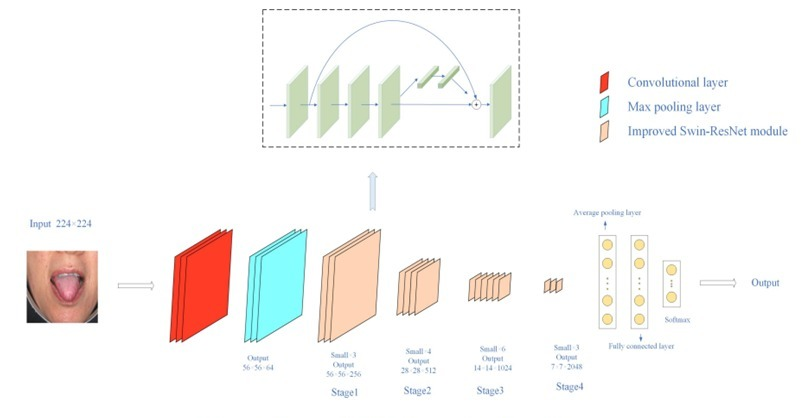
\includegraphics[width=0.80\textwidth]{2/figures/1.jpeg}
		\caption[Metodologia ResNet-50 and Swin Transformer]{Metodologia ResNet-50 and Swin Transformer. \\
		Fuente: \cite{Zhao2024}. \textit{Swin-ResNet: Research and Implementation of a Tooth-Marked
		Tongue Classification Method Combining ResNet-50 and Swin Transformer.}.}
		\label{2:fig123}
	\end{center}
\end{figure}

\cite{Tang2020} desarrollaron un enfoque innovador basado en aprendizaje profundo para la detección automática de lenguas con marcas de dientes, un elemento crucial en el diagnóstico dentro de la medicina tradicional china. El reto principal en este campo radica en la variabilidad de las características visibles de la lengua, particularmente en las marcas dejadas por los dientes en los bordes de la lengua, lo que requiere una metodología de clasificación altamente detallada y precisa. Para abordar este desafío, el equipo implementó una red neuronal convolucional en cascada, compuesta por tres etapas: coarse-Net, fine-Net y refine-Net, que trabajan conjuntamente para detectar y localizar la región de la lengua y los puntos de referencia clave asociados a las marcas dentales. Posteriormente, se emplearon redes ResNet-50 y VGG-16 para llevar a cabo una clasificación precisa de las imágenes de la lengua.

El conjunto de datos utilizado para entrenar y validar este modelo incluyó un total de 1,858 imágenes de lenguas, obtenidas del Hospital Afiliado de la Universidad de Medicina Tradicional China de Chengdu. La implementación de este sistema de aprendizaje profundo mostró una mejora significativa en las métricas de evaluación, superando los enfoques tradicionales que no emplean aprendizaje profundo en cuanto a precisión y consistencia con la percepción humana. El F1-score, que es una medida clave en la evaluación de modelos de clasificación, alcanzó un valor de 0.924 al utilizar ResNet-50, y mejoró aún más a 0.948 cuando se utilizó VGG-16. Estos resultados demostraron que la inclusión de la localización de la región de la lengua y los puntos de referencia de la lengua mejoró significativamente la precisión del modelo.

Este trabajo no solo resalta el potencial del aprendizaje profundo en el ámbito de la medicina tradicional china, sino que también establece un nuevo estándar en la clasificación de lenguas con marcas dentales, destacándose por su capacidad para realizar diagnósticos más rápidos y precisos que los métodos convencionales. La propuesta de \cite{Tang2020} representa un avance pionero en la integración de tecnologías avanzadas de reconocimiento visual para la mejora de diagnósticos médicos en este campo.

La metodología que se empleó para este trabajo fue la siguiente y se puede observar en la Figura \ref{2:fig124}.

\begin{figure}[H]
	\begin{center}
		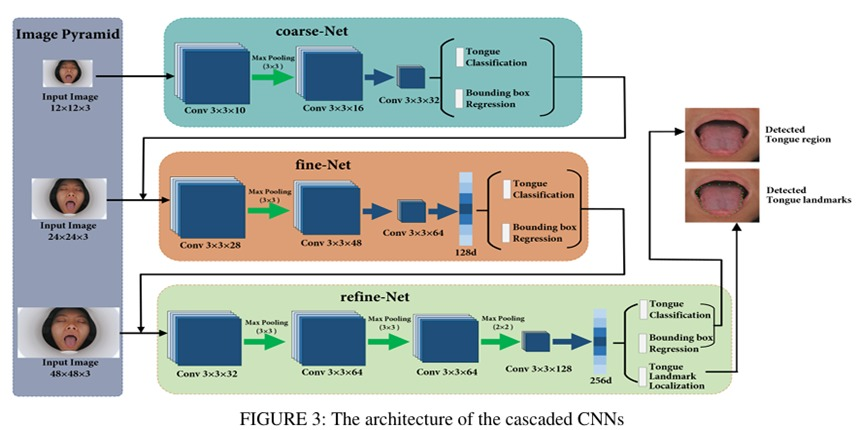
\includegraphics[width=0.80\textwidth]{2/figures/2.jpeg}
		\caption[Metodología ResNet-50 y VGG-16]{Metodología ResNet-50 y VGG-16. \\
		Fuente: \cite{Tang2020}. \textit{An Automatic Recognition of Tooth-Marked Tongue Based on Tongue Region Detection and Tongue Landmark Detection via Deep Learning.}.}
		\label{2:fig124}
	\end{center}
\end{figure}

La investigación llevada a cabo por \cite{Jiatuo2024} aborda el uso de algoritmos de aprendizaje profundo en el análisis y diagnóstico de imágenes de la lengua, un campo crucial en la medicina tradicional china (TCM). Este estudio se centra en el empleo del dataset público BioHit, que contiene 300 imágenes clínicas de lenguas, como base para la experimentación. A través del uso de redes neuronales convolucionales (CNNs) y técnicas de aprendizaje clásico, los autores lograron establecer un marco analítico que combina segmentación, detección de lesiones y clasificación automática de características presentes en las imágenes de lengua.  

En cuanto a la metodología, los investigadores implementaron una red neuronal profunda basada en CNN para extraer características específicas de las imágenes, enfocándose en patrones distintivos como marcas dentales, irregularidades en la textura y variaciones en el revestimiento de la lengua. Este enfoque permitió no solo identificar lesiones con precisión, sino también segmentar regiones clave de interés dentro de las imágenes. Paralelamente, se exploraron modelos clásicos para contrastar los resultados obtenidos con las técnicas más avanzadas.

El estudio reportó resultados significativos al comparar los enfoques clásicos con los de aprendizaje profundo. Mientras que los métodos convencionales alcanzaron una precisión aproximada del 80\% en la detección de lenguas marcadas por dientes, los modelos de aprendizaje profundo lograron precisiones mucho más altas, variando entre el 88\% y el 98.94\%. Entre los modelos más destacados se encuentran ResNet34, con una precisión máxima de 91.47\%, y una red neuronal convolucional multitarea, que alcanzó una precisión sobresaliente del 98.94\%. Este trabajo resalta cómo las técnicas basadas en inteligencia artificial no solo superan a los métodos tradicionales, sino que también aportan un nivel de estandarización y precisión nunca antes visto en el diagnóstico visual en TCM, abriendo nuevas posibilidades para el uso clínico de estas tecnologías.

La metodología seguida en este trabajo puede observarse en la Figura \ref{2:fig125}, la cual resume el proceso desde la segmentación inicial hasta la clasificación final basada en redes neuronales profundas.

\begin{figure}[H]
	\begin{center}
		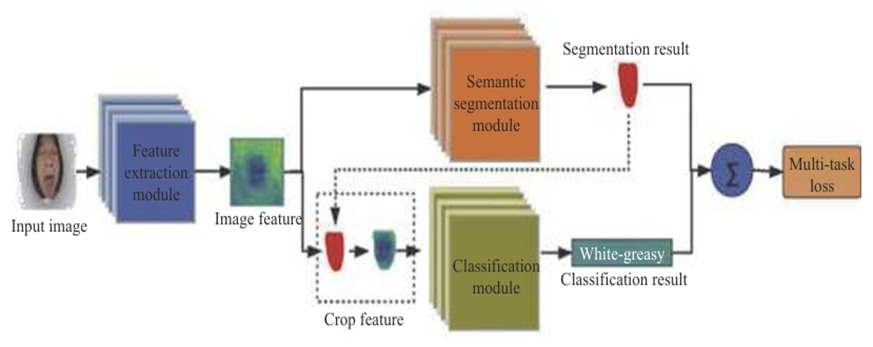
\includegraphics[width=0.80\textwidth]{2/figures/3.jpeg}
		\caption[Metodología de análisis de imágenes de lengua con CNNs]{Metodología de análisis de imágenes de lengua con CNNs. \\
		Fuente: \cite{Jiatuo2024}. \textit{Research status and prospect of tongue image diagnosis analysis based on machine learning.}.}
		\label{2:fig125}
	\end{center}
\end{figure}

En el trabajo de \cite{Liu2023}, se presenta un análisis exhaustivo sobre el uso de la inteligencia artificial en el diagnóstico médico mediante imágenes de lengua, un área relevante en la medicina tradicional china (TCM). A través de una revisión de los estudios más recientes publicados en bases de datos científicas como Web of Science y IEEE en los últimos cinco años, los autores destacan la evolución y los resultados prometedores obtenidos mediante la aplicación de algoritmos de aprendizaje profundo y técnicas híbridas. Este enfoque ha permitido avances significativos en la segmentación, detección y clasificación de imágenes de lengua, optimizando su uso en la diferenciación de síndromes y el diagnóstico de enfermedades.  

La metodología empleada se basa principalmente en el uso de redes neuronales convolucionales (CNNs) y modelos híbridos que integran inteligencia artificial con principios de TCM. Los modelos investigados incluyen técnicas avanzadas como ResNet50 y XGBT optimizado, los cuales se utilizaron para tareas específicas como la calibración y segmentación precisa de regiones de interés en las imágenes de lengua. Además, se destaca la implementación de modelos multitarea, como U-Net, que mejoraron significativamente la capacidad de detección y clasificación de lesiones, incrementando la eficiencia del diagnóstico.  

En términos de resultados, los modelos de aprendizaje profundo lograron precisiones que oscilan entre el 85\% y el 98\% en segmentación y clasificación de enfermedades a partir de imágenes de lengua. Por ejemplo, ResNet50 mostró una precisión de hasta el 92\% en la identificación de condiciones como prediabetes y diabetes. Por otro lado, los modelos híbridos, como un XGBT optimizado, alcanzaron un rendimiento máximo de 98\%, superando a métodos tradicionales en múltiples aspectos. Estas cifras resaltan la capacidad de la inteligencia artificial para transformar el diagnóstico médico al ofrecer mayor precisión y consistencia en los análisis visuales.

Pese a estos avances, los autores también subrayan desafíos importantes que persisten en esta área. Entre ellos se encuentran la necesidad de construir conjuntos de datos más completos y diversos, así como garantizar la fiabilidad en la evaluación de resultados. Además, se menciona que las futuras investigaciones deberían enfocarse en métodos de auto-supervisión y la fusión multimodal de datos, que permitirían una integración más robusta y precisa de la inteligencia artificial en los procesos de diagnóstico médico. Este trabajo establece una base sólida para el desarrollo continuo de tecnologías de diagnóstico inteligente basadas en imágenes de lengua, alineando la medicina tradicional con herramientas modernas de análisis.  

La metodología analizada en este estudio se ilustra en la Figura \ref{2:fig126}, la cual detalla el flujo de trabajo desde la segmentación inicial hasta la clasificación utilizando redes neuronales y modelos híbridos.

\begin{figure}[H]
	\begin{center}
		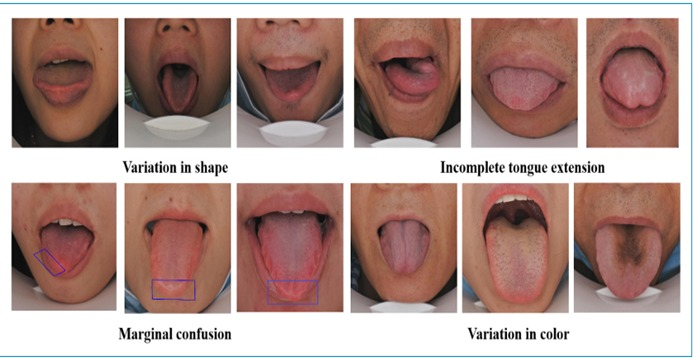
\includegraphics[width=0.80\textwidth]{2/figures/4.jpeg}
		\caption[Enfoque metodológico en el análisis de imágenes de lengua]{Enfoque metodológico en el análisis de imágenes de lengua utilizando modelos híbridos. \\
		Fuente: \cite{Liu2023}. \textit{A survey of artificial intelligence in tongue image for disease diagnosis and syndrome differentiation.}.}
		\label{2:fig126}
	\end{center}
\end{figure}

El estudio realizado por \cite{Jiang2022} examina la aplicación de algoritmos de aprendizaje profundo para el análisis de imágenes de lengua, integrando conocimientos de la medicina tradicional china (TCM). Con un conjunto de datos compuesto por 8,676 imágenes, estas fueron clasificadas en siete categorías distintas: lengua fisurada, marcada por dientes, estasis, con manchas, recubrimiento graso, pelada y podrida. Estas imágenes fueron recopiladas y anotadas por expertos en TCM, lo que garantiza la precisión y relevancia de los datos utilizados.  

La metodología principal implementada en este estudio se basa en el modelo Faster R-CNN, combinado con ResNet101 como extractor de características. Este enfoque permitió la detección y clasificación multietiqueta de las imágenes de lengua con un alto nivel de detalle. Para entrenar el modelo, las imágenes se dividieron en conjuntos de entrenamiento, validación y prueba, y se ejecutaron en un entorno optimizado con GPUs para acelerar los procesos de cálculo. Esta configuración permitió identificar patrones específicos en las imágenes, vinculándolos con características fisiológicas relevantes.  

En cuanto a los resultados, el modelo logró un desempeño destacado, alcanzando una precisión promedio del 90.67\%, una precisión puntual del 99.28\%, un recall del 91.25\% y un F1-score del 95.00\%. Estos indicadores destacan la capacidad del modelo para identificar con precisión características complejas y relevantes en las imágenes de lengua. Además, en una aplicación diagnóstica más amplia, el modelo identificó características específicas en una población de análisis, como lenguas fisuradas (41.49\%), marcadas por dientes (37.16%) y con recubrimiento graso (29.66\%).  

Más allá de la clasificación precisa, el estudio reveló asociaciones significativas entre las características de la lengua y ciertas condiciones metabólicas, como hipertensión, sobrepeso y enfermedades relacionadas con el hígado graso no alcohólico (NAFLD). Estas correlaciones sugieren que las características visibles de la lengua pueden ser indicadores valiosos para diagnósticos tempranos en diversas enfermedades. Asimismo, se identificaron variaciones en la prevalencia de estas características según el género y la edad de los individuos, lo que subraya la importancia de personalizar los análisis diagnósticos.  

\begin{figure}[H]
	\begin{center}
		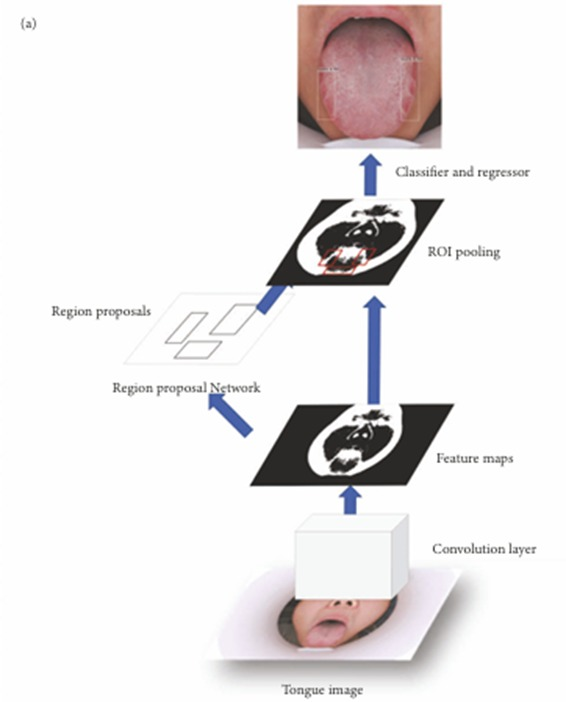
\includegraphics[width=0.7\textwidth]{2/figures/5.jpeg}
		\caption[Metodología con Faster R-CNN y ResNet101]{Metodología con Faster R-CNN y ResNet101 para el análisis de imágenes de lengua. \\
		Fuente: \cite{Jiang2022}. \textit{Deep learning analysis of tongue images in traditional Chinese medicine diagnosis.}.}
		\label{2:fig127}
	\end{center}
\end{figure}

El estudio presentado por \cite{Feasibility2020} analiza la viabilidad de Google’s Teachable Machine (versión 2.0) como herramienta de aprendizaje automático para el diagnóstico de lenguas marcadas por dientes, una característica comúnmente asociada con diversas afecciones de salud bucal. Utilizando un conjunto de datos de 1,250 imágenes obtenidas de Kaggle, el estudio incluye 704 imágenes de lenguas con marcas de dientes y 546 sin marcas, recopiladas y etiquetadas para garantizar su adecuación en aplicaciones diagnósticas.

La metodología se centró en optimizar el rendimiento del modelo ajustando hiperparámetros clave como el número de épocas, el tamaño del lote y la tasa de aprendizaje. El conjunto de datos se dividió en un 90\% para entrenamiento y un 10\% para pruebas, asegurando un adecuado equilibrio entre generalización y precisión. Google’s Teachable Machine, diseñada para simplificar la implementación de modelos de aprendizaje automático, fue utilizada como herramienta base, demostrando que su interfaz accesible puede integrarse en flujos de trabajo clínicos para diagnóstico.

Los resultados obtenidos muestran que el modelo logró una precisión del 92.1\% en la identificación de lenguas marcadas por dientes, mientras que para lenguas sin marcas alcanzó un 72.6\%. La sensibilidad del modelo fue de 0.92, destacando su capacidad para detectar correctamente casos positivos, aunque la especificidad fue baja (0.28), indicando limitaciones en la identificación de casos negativos. Este rendimiento supera al de estudios previos basados en redes neuronales convolucionales más complejas, lo que subraya la efectividad de herramientas accesibles como Teachable Machine en contextos clínicos.

Estos hallazgos no solo resaltan la capacidad de esta herramienta para realizar diagnósticos con una precisión competitiva, sino que también abren la puerta a nuevas aplicaciones en entornos con recursos limitados, donde el acceso a infraestructura avanzada de aprendizaje profundo es restringido. Además, el enfoque simplificado de Google’s Teachable Machine facilita la adopción de tecnologías de inteligencia artificial en la práctica médica, permitiendo a los profesionales implementar soluciones rápidas y eficientes para el diagnóstico de condiciones clínicas.

\begin{figure}[H]
	\begin{center}
		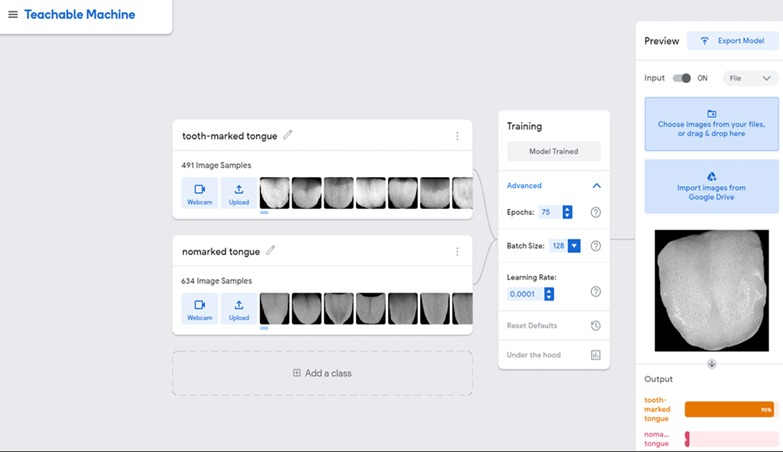
\includegraphics[width=0.80\textwidth]{2/figures/6.jpeg}
		\caption[Flujo de trabajo en Google’s Teachable Machine]{Flujo de trabajo para diagnóstico de lengua marcada por dientes utilizando Google’s Teachable Machine. \\
		Fuente: \cite{Feasibility2020}. \textit{Feasibility Study of Google's Teachable Machine in Diagnosis of Tooth-Marked Tongue.}.}
		\label{2:fig128}
	\end{center}
\end{figure}

El estudio de \cite{Kong2020} presenta una metodología avanzada para la detección y análisis de lenguas marcadas por dientes, un rasgo distintivo en el diagnóstico de la medicina tradicional china (TCM), que puede estar asociado con disfunciones en órganos internos como el hígado y el bazo. Este trabajo se basa en un conjunto de datos compuesto por 1,500 imágenes clínicas de alta calidad provenientes del Hospital Shu Guang en Shanghái. Dentro de este conjunto, se seleccionaron específicamente 400 imágenes de lenguas normales y 756 con marcas de dientes, las cuales fueron etiquetadas manualmente para garantizar la precisión en la segmentación y localización de las marcas.

La metodología empleada combina el poder del modelo Mask Scoring R-CNN con técnicas de aprendizaje por transferencia, utilizando ResNet-101 como red base. Este enfoque permitió una segmentación precisa y una localización detallada de las marcas dentales presentes en las imágenes. Antes del entrenamiento del modelo, las imágenes fueron sometidas a un proceso de preprocesamiento intensivo, incluyendo la normalización del color, recorte y etiquetado manual de las áreas de interés para generar máscaras altamente detalladas. Estos pasos fueron fundamentales para optimizar la detección de marcas dentales, especialmente en casos con grados de severidad diversos.

Los resultados del estudio fueron sobresalientes. El modelo alcanzó un F1-score de 0.95, lo que refleja un equilibrio casi perfecto entre precisión y recall. Además, la precisión específica del modelo fue del 99\%, mientras que el recall alcanzó un valor notable de 91.4\%. Estos indicadores demuestran no solo la alta precisión del modelo, sino también su capacidad para generalizar en diferentes escenarios clínicos. Esto es particularmente relevante dado que las lenguas marcadas por dientes pueden variar significativamente en términos de su apariencia y severidad.

Una de las contribuciones más destacadas de esta investigación es su aplicabilidad en el ámbito de la telemedicina. Al integrar herramientas avanzadas de aprendizaje profundo como Mask Scoring R-CNN, se abre la posibilidad de realizar diagnósticos detallados a distancia, reduciendo la dependencia de evaluaciones presenciales y facilitando el acceso a servicios médicos especializados. Esto es especialmente relevante en áreas donde la medicina tradicional china es una práctica común, pero los recursos médicos pueden ser limitados.

\begin{figure}[H]
	\begin{center}
		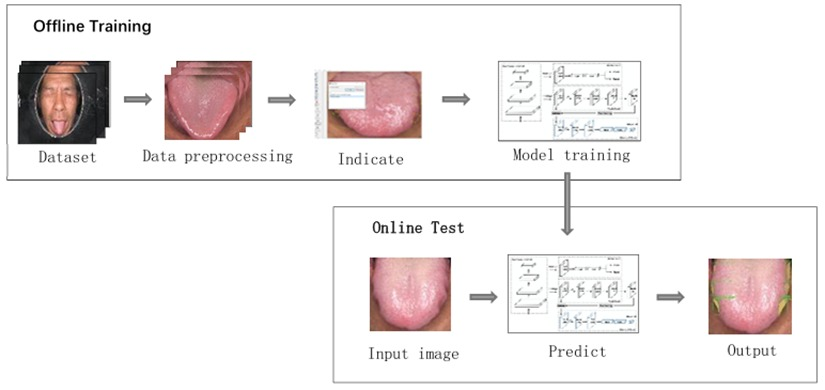
\includegraphics[width=0.80\textwidth]{2/figures/7.jpeg}
		\caption[Detección de lengua marcada por dientes con Mask Scoring R-CNN]{Esquema de segmentación y localización de marcas dentales utilizando Mask Scoring R-CNN con ResNet-101. \\
		Fuente: \cite{Kong2020}. \textit{Tooth-marked tongue recognition based on Mask Scoring R-CNN.}}
		\label{2:fig129}
	\end{center}
\end{figure}

Este estudio subraya la relevancia de la inteligencia artificial en la modernización de los diagnósticos basados en imágenes, mostrando cómo modelos avanzados pueden superar las limitaciones tradicionales de precisión y consistencia en el análisis de características complejas como las marcas de dientes en la lengua.

El trabajo de \cite{Tiryaki2024} explora el uso de redes neuronales profundas (DCNN) en la identificación y clasificación de lesiones en la lengua, un campo emergente con importantes aplicaciones clínicas. Este estudio aborda específicamente cinco categorías: lengua normal y cuatro tipos de lesiones comunes, incluyendo lengua fisurada, lengua geográfica, lengua recubierta y glositis romboidal mediana. Para este análisis, se recopiló un conjunto de datos compuesto por 623 imágenes clínicas de lengua, etiquetadas de manera experta para garantizar la precisión en la categorización.

La metodología implementada incluyó el uso de varios modelos avanzados de DCNN, como VGG19, ResNet50, ResNet101 y GoogLeNet. Estos modelos se beneficiaron del aprendizaje por transferencia, una técnica que aprovecha redes preentrenadas para mejorar la eficiencia en problemas con datos limitados. Además, este estudio introdujo por primera vez en este contexto un enfoque innovador basado en la fusión por votación mayoritaria (FBMV, por sus siglas en inglés), diseñado para combinar las predicciones de múltiples modelos y mejorar la precisión global.

Los resultados obtenidos fueron notables tanto en la clasificación binaria como en la clasificación multiclase. En la tarea binaria (lengua normal vs. lengua con lesiones), el modelo ResNet101 logró una precisión inicial del 93.53\%. Este rendimiento fue mejorado significativamente mediante la aplicación del enfoque FBMV, alcanzando un 95.15\%. Para la clasificación multiclase, que abarcó las cinco categorías, VGG19 se destacó con una precisión del 83.93\%, la cual fue incrementada al 88.76\% tras incorporar FBMV. Estos resultados no solo demuestran la robustez de las redes neuronales profundas en la detección de características complejas de la lengua, sino también el valor añadido del enfoque de fusión para abordar problemas de clasificación con múltiples clases.

Además de los resultados cuantitativos, el estudio subraya el potencial de estas tecnologías en el ámbito clínico. La capacidad de las DCNN para identificar patrones sutiles y correlaciones en imágenes médicas abre nuevas posibilidades para diagnósticos automatizados y personalizados. Este avance es especialmente relevante en entornos con recursos limitados, donde las herramientas basadas en inteligencia artificial pueden complementar la experiencia de los profesionales de la salud, mejorando la eficiencia y reduciendo los tiempos de diagnóstico.

\begin{figure}[H]
	\begin{center}
		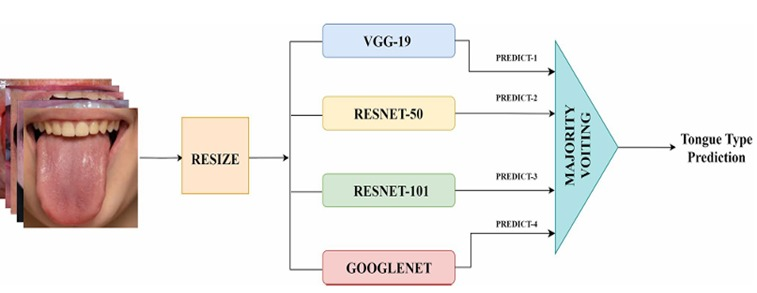
\includegraphics[width=0.85\textwidth]{2/figures/8.jpeg}
		\caption[Clasificación de lesiones linguales con DCNN y FBMV]{Estrategia de fusión por votación mayoritaria aplicada a modelos DCNN para clasificaciones binaria y multiclase. \\
		Fuente: \cite{Tiryaki2024}. \textit{Artificial intelligence in tongue diagnosis: classification of tongue lesions and normal tongue images using deep convolutional neural network.}}
		\label{2:fig130}
	\end{center}
\end{figure}

En conclusión, este trabajo destaca cómo la integración de DCNN y enfoques innovadores como FBMV puede transformar el diagnóstico de enfermedades bucales, proporcionando una base sólida para investigaciones futuras y desarrollos tecnológicos en medicina basada en imágenes.


\section{Bases Teóricas}
\subsection{Bruxismo en niños}

\subsubsection{Definición}

El término "bruxismo" proviene del griego "brygmós", que significa "apretar o rechinar los dientes". Este trastorno, también conocido como la "enfermedad silenciosa", afecta aproximadamente al 70\% de los pacientes, y su aparición se vincula principalmente al estrés y problemas psicológicos \parencite{Rojas2022}. Según lo descrito por \textcite{Rojas2022}, el bruxismo representa un desafío común en la salud dental a nivel mundial, generando alteraciones en el aparato masticatorio y contribuyendo a cambios morfológicos que comprometen la salud bucal.

Es importante destacar que el término "bruxismo" suele confundirse con otros relacionados, como bruxismo céntrico, excéntrico, nocturno, diurno, bruxomanía, parafunción, apretamiento dentario, rechinamiento dentario, entre otros \parencite{Zambra2003}.

\subsubsection{Síntomas}

Los síntomas del bruxismo en niños incluyen sonidos audibles durante el acto de apretar o rechinar los dientes, ya sea consciente o inconscientemente. Estos pueden manifestarse como chasquidos o movimientos dentales en posición céntrica o excéntrica, durante actividades como la deglución o masticación, tanto de día como de noche \parencite{vallejo2002bruxismoinfantil}. 

La magnitud de los síntomas depende de la resistencia de las estructuras involucradas y de factores como la duración, frecuencia e intensidad del bruxismo. Aunque algunas estructuras del sistema masticatorio absorben estas fuerzas sin consecuencias, otras experimentan daños que van desde el desgaste dental hasta alteraciones en los músculos masticatorios y las articulaciones temporomandibulares \parencite{vallejo2002bruxismoinfantil}.

\subsubsection{Factores de riesgo}

\paragraph{Factores odontológicos}  
El bruxismo puede estar influido por condiciones como maloclusiones esqueléticas, alteraciones oclusales y restauraciones dentales defectuosas. Sin embargo, los estudios en este ámbito han arrojado resultados inconsistentes \parencite{Zambra2003}.

\paragraph{Factores psicológicos}  
El estrés y la ansiedad son factores psicológicos clave asociados al bruxismo, especialmente en adolescentes. Un estudio indicó que los niveles elevados de catecolaminas en la orina de niños de 6 a 8 años podrían estar relacionados con altos niveles de ansiedad \parencite{vanderas1999catecholaminebruxism}. Sin embargo, otros factores como el nivel socioeconómico y cultural no muestran resultados concluyentes \parencite{serranegra2009psychosocialbruxism}.

\paragraph{Factores relacionados con el sueño}  
El bruxismo nocturno, considerado una parasomnia, ocurre durante el sueño y está relacionado con despertares parciales y altos niveles de estrés emocional. Aunque estas alteraciones son comunes en la infancia, su frecuencia persistente puede indicar problemas psicológicos subyacentes \parencite{vieiraandrade2014sleepbruxism}.

\paragraph{Factores genéticos}  
Evidencia sugiere que el bruxismo puede tener una base genética, ya que los niños cuyos padres presentaron bruxismo tienen mayor probabilidad de desarrollarlo, lo que señala una predisposición hereditaria \parencite{hublin2001parasomniasgenetics}.

\subsection{Diagnóstico y prediagnóstico del bruxismo}

\subsubsection{Método instrumental}  
La polisomnografía es considerada la técnica de referencia para diagnosticar el bruxismo durante el sueño, ya que permite un monitoreo completo de la actividad cerebral, muscular y respiratoria. Asimismo, los registros electromiográficos (EMG) y las aplicaciones móviles emergen como herramientas innovadoras para evaluar la actividad muscular en tiempo real \parencite{gutierrez2021bruxismorino}.

\subsubsection{Método no instrumental}  
El diagnóstico mediante autorreporte y evaluación clínica es ampliamente utilizado debido a su accesibilidad y bajo costo. Sin embargo, estos métodos presentan limitaciones en comparación con los instrumentales, por lo que su precisión aún debe ser mejorada \parencite{gutierrez2021bruxismorino}.

\subsection{Aprendizaje profundo y visión por computadora}

\subsubsection{Definición}  
El aprendizaje profundo, según \textcite{kim2017matlabdeeplearning}, se basa en redes neuronales con múltiples capas ocultas. Estas estructuras permiten procesar datos complejos de manera jerárquica, lo que constituye la esencia del Deep Learning.

\subsubsection{Visión por computadora}  
La visión por computadora busca replicar la capacidad humana de interpretar información visual a través de algoritmos y modelos matemáticos. Este campo, iniciado por David Marr en la década de 1980, ha evolucionado hacia aplicaciones que abarcan desde la robótica hasta el diagnóstico médico \parencite{szeliski2010computervision}.

\subsubsection{Aplicación en la salud}  
En medicina, la visión por computadora permite detectar patrones y anomalías en imágenes médicas como radiografías y resonancias magnéticas. Por ejemplo, las redes neuronales convolucionales han demostrado ser eficaces en la identificación de tumores, mejorando la velocidad y precisión del diagnóstico \parencite{litjens2017deeplearningmedical}.

\subsection{Aplicaciones móviles}

\subsubsection{Definición}  
Las aplicaciones móviles son programas diseñados para dispositivos como smartphones y tablets, ofreciendo una amplia gama de funcionalidades que van desde el entretenimiento hasta la salud \parencite{marinescu2019mobileappdev}.

\subsubsection{Importancia en la salud}  
Estas aplicaciones han revolucionado la gestión de la salud al ofrecer herramientas personalizadas para el monitoreo, la consulta y la toma de decisiones informadas. Además, promueven la autonomía de los pacientes al proporcionar acceso inmediato a información confiable \parencite{marinescu2019mobileappdev}.


\section{Marco Conceptual}
\subsection{Bruxismo primario}
El bruxismo primario, también conocido como idiopático, es un trastorno caracterizado por el hábito inconsciente de apretar o rechinar los dientes, especialmente durante el sueño. A diferencia del bruxismo secundario, no se asocia a una causa médica o psicológica identificable. Se cree que factores genéticos, estrés y trastornos del sueño podrían estar involucrados en su desarrollo. A largo plazo, el bruxismo primario puede causar desgaste dental, dolor en la mandíbula y otros problemas bucales \parencite{kato2001epidemiologybruxism}.

\subsection{Disfunción temporomandibular}
La disfunción temporomandibular (DTM) se caracteriza por diversos síntomas, incluyendo dolor en la región bucal, sonidos en las articulaciones y restricciones en los movimientos de la mandíbula. Esta condición tiene múltiples causas, que abarcan desde traumatismos y hábitos parafuncionales hasta el estrés, todos los cuales pueden exceder la capacidad fisiológica de los individuos. Factores como la estabilidad articular, la oclusión dental y características genéticas también son determinantes. Un estudio indica que hay una relación entre el bruxismo durante el sueño y la presencia de dolor en pacientes con DTM, lo que enfatiza la necesidad de una evaluación exhaustiva para su tratamiento \parencite{blanco2014selfreportbruxism}.

\subsection{Cefaleas}
Las cefaleas son uno de los trastornos más frecuentes del sistema nervioso, afectando a aproximadamente la mitad de los adultos en el último año y siendo la sexta causa de incapacidad en el mundo. Aunque la mayoría no son graves, es importante buscar atención médica si el dolor es intenso y repentino, o si se acompaña de síntomas neurológicos o fiebre \parencite{clinica2018cefalea}.

\subsection{Sensibilidad dental}
La hipersensibilidad dentinaria (HD), también conocida como sensibilidad dental, se caracteriza por un dolor intenso y temporal en los dientes, que ocurre debido a la exposición de la dentina al entorno bucal. Este tipo de dolor se desencadena por estímulos externos como alimentos o bebidas frías, calientes, ácidas o dulces, así como por la presión táctil \parencite{dentaid2024sensibilidad}.

\subsection{Odontología del sueño}
La medicina dental del sueño es una especialidad odontológica que se ocupa del tratamiento de los trastornos del sueño, siendo el síndrome de apnea obstructiva del sueño (SAOS) y los ronquidos las afecciones más comunes tratadas \parencite{gutierrez2021bruxismorino}.

\subsection{Lingua geográfica}
La lengua geográfica es una condición inflamatoria que, aunque no representa un riesgo, se manifiesta en la superficie de la lengua. En esta afección, la lengua presenta pequeñas protuberancias de color blanco rosado, conocidas como papilas, que son estructuras finas similares a vellos. En las áreas afectadas por la lengua geográfica, las papilas están ausentes, dejando zonas suaves y rojas, a menudo con bordes ligeramente elevados \parencite{mayoclinic2024lenguageografica}.

\subsection{Redes neuronales convolucionales}
\subsubsection{Definición y funcionamiento}
Las redes neuronales convolucionales (CNN) son un tipo de red neuronal organizadas en varias capas, conocidas como multicapa. Estas redes presentan una arquitectura donde las neuronas están interconectadas. 

\subsubsection{Componentes principales}
Se componen de una capa de convolución, donde cada neurona filtra la información de entrada para generar un mapa de características; seguida por una capa de submuestreo, que reduce el tamaño de la información procesada; y finalmente, una capa completamente conectada que se encarga de la clasificación. Las CNN son especialmente eficaces en proyectos de procesamiento de imágenes gracias a su capacidad de clasificación \parencite{lopezpacheco2021redesconv}.

\subsection{Support Vector Machines (SVM)}
Las Support Vector Machines son un conjunto de métodos de aprendizaje supervisado utilizados para clasificación y regresión. Se basan en encontrar un hiperplano óptimo que separa diferentes clases en un espacio multidimensional. Este hiperplano maximiza el margen entre las clases más cercanas, llamadas vectores de soporte. Las SVM son efectivas en espacios de alta dimensión y pueden utilizarse con distintos tipos de núcleos (kernels) para manejar problemas no lineales \parencite{cortes1995svm}.

\subsection{Extracción de características}
La extracción de características es el proceso de transformar datos en bruto y complejos en representaciones numéricas más simples y significativas, llamadas características. Estas características son luego utilizadas como entrada para algoritmos de aprendizaje automático, permitiendo a las máquinas "entender" y aprender de los datos \parencite{szeliski2010computervision}.

\subsection{Transfer learning}
El \textit{transfer learning} permite utilizar modelos preentrenados en un nuevo conjunto de datos, facilitando la mejora del rendimiento cuando se dispone de pocos datos. Esto ahorra tiempo y recursos durante el entrenamiento, aprovechando el conocimiento previo \parencite{pan2010survey}.

\subsection{Data augmentation}
El \textit{data augmentation} amplía un conjunto de datos mediante transformaciones como rotaciones y escalados. Esta técnica mejora la robustez del modelo y reduce el riesgo de sobreajuste, creando un conjunto más diverso para el entrenamiento \parencite{shorten2019survey}.

\subsection{Segmentación de imágenes}
La segmentación de imágenes divide una imagen en regiones significativas para facilitar la identificación de objetos. Es esencial en tareas de detección y reconocimiento, utilizando redes neuronales para lograr alta precisión \parencite{litjens2017deeplearningmedical}.

\subsection{Redes generativas adversarias}
Las redes generativas adversarias (GANs) consisten en un generador y un discriminador que compiten entre sí. El generador crea datos sintéticos, mientras que el discriminador evalúa su autenticidad. Son efectivas en la generación de imágenes y la mejora de resolución \parencite{goodfellow2014generative}.

\subsection{Pooling}
El \textit{pooling} es una técnica utilizada en redes neuronales convolucionales (CNN) para reducir la dimensionalidad de los mapas de características generados por las capas de convolución. Este proceso consiste en aplicar una función de agregación, como la máxima (\textit{max pooling}) o la media (\textit{average pooling}), sobre bloques de características. Ayuda a disminuir la carga computacional, mejora la generalización del modelo y hace que las redes sean menos sensibles a pequeñas variaciones en la entrada \parencite{boureau2010theoretical}.

\subsection{Regularización}
La regularización previene el sobreajuste en modelos de aprendizaje automático. Incluye técnicas como la penalización de coeficientes y el \textit{dropout}, que apaga neuronas aleatoriamente durante el entrenamiento para mejorar la generalización del modelo \parencite{srivastava2014dropout}.


\section{Hipótesis}
\subsection{Hipótesis General}
HG: \newcommand{\HipotesisGeneral}{
	El uso de un sistema automatizado basado en técnicas de aprendizaje profundo, como las redes neuronales convolucionales (CNN), permite realizar un prediagnóstico efectivo del bruxismo en niños mediante la identificación de patrones visuales en imágenes de la lengua, con una precisión comparable o superior a los métodos diagnósticos tradicionales.
	}
\HipotesisGeneral


\subsection{Hipótesis Específicas}
\newcommand{\Hone}{
	Un modelo de aprendizaje profundo, específicamente una red neuronal convolucional (CNN), puede clasificar imágenes de la lengua con alta precisión para detectar signos de bruxismo en niños.
	}
\newcommand{\Htwo}{
	Existen patrones visuales distintivos en las imágenes de la lengua que están relacionados con episodios de bruxismo en niños.
	}
\newcommand{\Hthree}{
	Las técnicas de procesamiento de imágenes, como la segmentación y el análisis de texturas, son efectivas para extraer características relevantes de las imágenes de la lengua para el diagnóstico de bruxismo.
	}
\newcommand{\Hfour}{
	El sistema automatizado basado en aprendizaje profundo logra una precisión, sensibilidad y especificidad competitivas en la detección de bruxismo en niños en comparación con los métodos tradicionales.
	}
\newcommand{\Hfive}{
	La implementación de un sistema automatizado para el análisis de imágenes de la lengua incrementa la tasa de detección temprana de bruxismo en niños, facilitando su diagnóstico en entornos clínicos y domésticos.
		}

\begin{itemize}
	\item HE1: {\Hone}
	\item HE2: {\Htwo}
	\item HE3: {\Hthree}
	\item HE4: {\Hfour}
	\item HE5: {\Hfive}
\end{itemize}

\chapter{Metodología de la Investigación}
\section{Diseño de la investigación}
El diseño de esta investigación es de tipo cuasi-experimental, ya que se observará la relación entre las marcas en los bordes de la lengua (variable independiente) y la presencia de bruxismo (variable dependiente) en niños, sin manipular el entorno ni asignar condiciones al azar. Las imágenes de las lenguas serán procesadas mediante técnicas de visión computacional para extraer características clave, que luego serán evaluadas mediante modelos de deep learning. Este enfoque permite analizar patrones asociados al bruxismo de forma controlada y sistemática, sin alterar las condiciones naturales de los participantes.

\subsection{Alcance de la investigación}
El nivel de esta investigación es explicativo, ya que se busca desarrollar una aplicación móvil que permita el prediagnóstico de bruxismo en niños mediante el análisis de imágenes de sus lenguas. El sistema de visión computacional que se propone está diseñado para identificar patrones específicos, como las marcas en los bordes de la lengua, los cuales podrían estar asociados a esta condición. Este enfoque permite establecer una relación de causa-efecto, donde la presencia de ciertos patrones en las imágenes analizadas puede servir como indicador preliminar de bruxismo, facilitando una detección temprana y preventiva.

\subsection{Enfoque de la investigación}
El enfoque de esta investigación es cuantitativo, ya que se busca obtener datos medibles para el prediagnóstico de bruxismo en niños. Para esto, se emplearán imágenes de lenguas de niños con posibles signos de bruxismo, específicamente marcas en los bordes, que serán procesadas mediante técnicas de visión computacional. Los resultados obtenidos serán datos numéricos que permitirán entrenar modelos de deep learning para identificar patrones asociados al bruxismo. Estos modelos se utilizarán como herramienta de apoyo para el prediagnóstico, aportando precisión y rapidez en la detección de esta condición en una etapa temprana.

\subsection{Población}
La población de esta investigación está constituida por individuos que presentan posibles señales de bruxismo, específicamente aquellos con marcas en los bordes de la lengua identificadas mediante examen visual o imágenes clínicas.

\subsection{Muestra}
La muestra utilizada en esta investigación consiste en un conjunto de 1250 imágenes de lenguas marcadas y no marcadas, obtenidas de la plataforma kaggle, de las cuales todas fueron tomadas de personas con posibles señales de bruxismo.

\section{Operacionalización de variables}
En este apartado se describen las principales variables del estudio, detallando su definición conceptual, definición operacional, los indicadores asociados, así como el instrumento y la escala utilizada para su medición. Estas variables permiten estructurar y guiar el proceso de análisis basado en técnicas de aprendizaje profundo.

\begin{table}[H]
\centering
\caption{Definición de variables del estudio.}
\label{tabla:variables}
\begin{tabular}{|p{2.5cm}|p{3cm}|p{3.5cm}|p{2.5cm}|p{2.5cm}|p{1.5cm}|}
\hline
\textbf{Variable} & \textbf{Definición Conceptual} & \textbf{Definición Operacional} & \textbf{Indicadores} & \textbf{Instrumento} & \textbf{Escala} \\ \hline
\textbf{Marcas en los bordes de la lengua} & Signos visuales en el borde de la lengua indicativos de bruxismo. & Detección de marcas en imágenes procesadas mediante técnicas de visión computacional. & Presencia o ausencia de marcas. & Modelo de \textit{deep learning}. & Nominal \\ \hline
\textbf{Presencia de bruxismo} & Apretamiento o rechinamiento involuntario de dientes, identificado por signos en lengua. & Diagnóstico preliminar basado en patrones visuales asociados al bruxismo. & Predicción del modelo. & Modelo de \textit{deep learning}. & Nominal \\ \hline
\end{tabular}
\end{table}

\section{Técnicas de recolección de datos}
En esta sección se describen las técnicas utilizadas para la obtención y el procesamiento de los datos necesarios para el desarrollo del modelo de aprendizaje profundo. Se detalla la fuente de datos, el proceso de recolección y las herramientas empleadas en el análisis.

\begin{table}[H]
    \caption{Técnicas de recolección de datos.}
    \centering
    \renewcommand{\arraystretch}{1.5} % Aumenta el espacio entre filas
    \setlength{\tabcolsep}{8pt} % Ajusta el espacio entre columnas
    \begin{tabular}{|p{4cm}|p{10cm}|}
        \hline
        \textbf{Técnica} & \textbf{Descripción} \\ \hline
        Fuente de datos & 1250 imágenes de lenguas marcadas y no marcadas obtenidas de Kaggle. \\ \hline
        Proceso de recolección & Selección, preprocesamiento y etiquetado de las imágenes para la detección de marcas indicativas de bruxismo. \\ \hline
        Herramientas utilizadas & Visión computacional para detección de características y \textit{deep learning} para análisis y clasificación de imágenes. \\ \hline
    \end{tabular}
\end{table}


\section{Metodología de Implementación de la Solución}

La metodología propuesta para implementar un modelo de \textit{Deep Learning} está basada en el ciclo de vida de desarrollo de modelos de Inteligencia Artificial, con adaptaciones específicas para abordar el diagnóstico de bruxismo en niños mediante patrones de sonido y frecuencia, así como el análisis de imágenes de lengua.

Para este caso, se busca desarrollar un modelo de \textit{Deep Learning} que asista en el prediagnóstico de bruxismo infantil. La metodología propuesta toma como referencia algunos enfoques presentados en los antecedentes revisados, adaptándolos para el análisis de datos de sonido y procesamiento de imágenes relacionadas con marcas en los bordes de la lengua. En la Figura \ref{3:fig301} se presenta de manera gráfica la metodología propuesta para este proyecto.

\begin{figure}[H]
	\begin{center}
		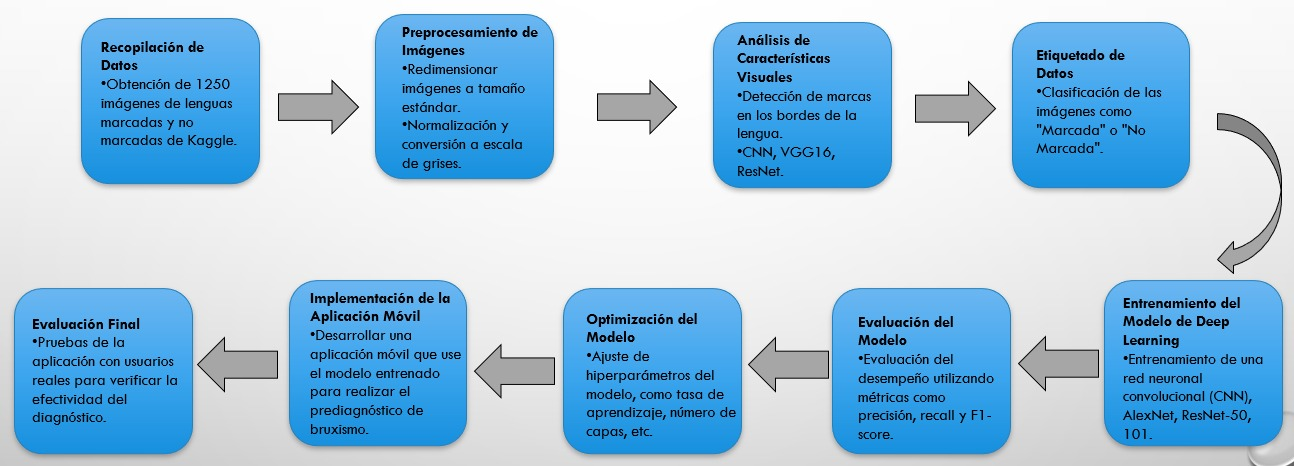
\includegraphics[width=1.00\textwidth]{3/figures/1.jpeg}
		\caption[Metodología de implementación]{Metodología de implementación. \\
		Fuente: Elaboración propia.}
		\label{3:fig301}
	\end{center}
\end{figure}





\input{4/desarrollo}
\input{5/resultados} %Esta es la conclusión
%\input{6/conclusion}
% %%Bibliografia
%\bibliographystyle{apalike} % No funciona
%\renewcommand{\bibname}{BIBLIOGRAFÍA} % changes the header; default: Bibliography

\printbibliography[heading=bibintoc,title={Referencias}]
%\bibliography{biblio/references} % adjust this to fit your BibTex file

%%Anexos
\appendix
\renewcommand{\appendixname}{Anexo} %Esto es para las paginas
\renewcommand{\appendixtocname}{Anexos} %Esto es para el indice
\renewcommand{\appendixpagename}{Anexos}
\clearpage
\addappheadtotoc
\appendixpage
%\begin{appendices}

\appendix
%\chapter*{ANEXOS}% If \appendix doesn't insert a \chapter
%\addcontentsline{toc}{chapter}{ANEXOS}% Print Appendix in ToC
\setcounter{section}{0}% Reset numbering for sections
\renewcommand{\thesection}{\Alph{section}}% Adjust section printing (from here onward)
	
	\section{Árbol de Problemas}
	%\chapter*{Árbol de Problemas}
	%\addcontentsline{toc}{section}{Árbol de Problemas}
	%\renewcommand{\thechapter}{A}
	\label{anexo1}
	\begin{figure}[h]
		\begin{center}
			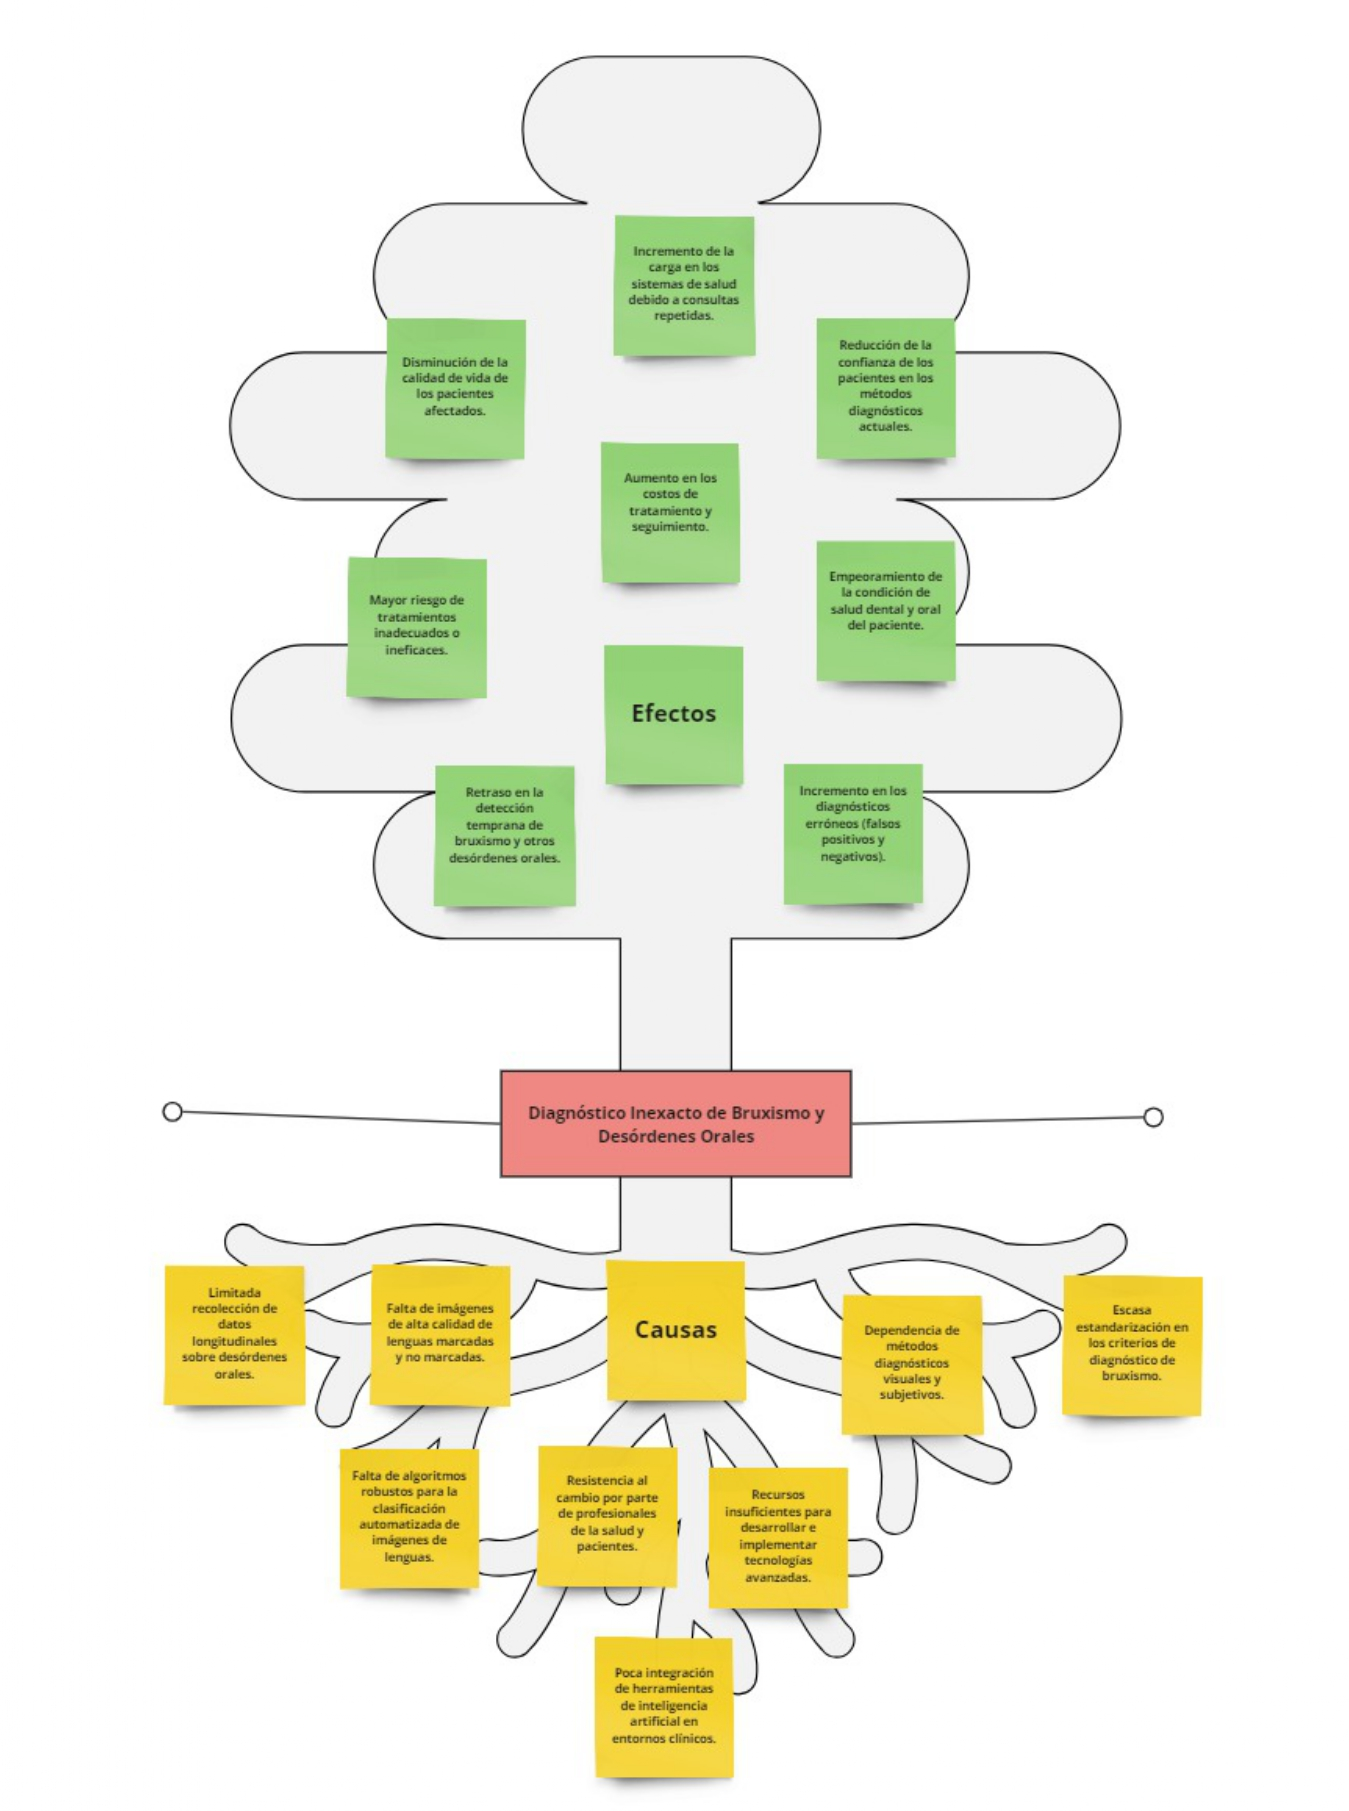
\includegraphics[width=0.85\textwidth]{anexos/arbol_problematica.jpg}
			%\caption{Fuente: Elaboración propia}
		\end{center}
	\end{figure}
	\clearpage

	\section{Matriz de contingencia}
\begin{table}[H]
    \caption{Problema, objetivos y variables de la investigación.}
    \centering
    \renewcommand{\arraystretch}{1.5} % Aumenta el espacio entre filas
    \setlength{\tabcolsep}{10pt} % Ajusta el espacio entre columnas
    \begin{tabular}{|p{4cm}|p{5cm}|p{6cm}|}
        \hline
        \textbf{Problema} & \textbf{Objetivo} & \textbf{Variables} \\ \hline
        \textbf{Principal:} ¿Cómo puede un sistema automatizado, basado en técnicas de aprendizaje profundo, realizar un prediagnóstico efectivo del bruxismo en niños? 
        & Desarrollar y validar un sistema automatizado basado en técnicas de aprendizaje profundo para el prediagnóstico de bruxismo en niños. 
        & 
        \textbf{Dependiente:} Precisión del prediagnóstico de bruxismo. \\
        & & \textbf{Independiente:} Técnicas de procesamiento de imágenes, patrones visuales. \\ \hline
        \textbf{Específicos:} 
        \begin{itemize}
            \item ¿Cuáles son los patrones visuales en imágenes de la lengua que están asociados con el bruxismo? 
            \item ¿Qué técnicas de procesamiento son más efectivas para identificar signos de bruxismo?
        \end{itemize} 
        & 
        \begin{itemize}
            \item Identificar patrones visuales en imágenes de la lengua indicativos de bruxismo infantil.
            \item Evaluar técnicas de procesamiento y extracción de características.
        \end{itemize} 
        & 
        \textbf{Dependiente:} Detección temprana de bruxismo. \\
        & & \textbf{Independiente:} Redes neuronales convolucionales (CNN), imágenes de la lengua. \\ \hline
    \end{tabular}
\end{table}

	
	\clearpage
\end{document}